\documentclass{sig-alternate}
\usepackage{graphicx}
\usepackage{balance}  % for  \balance command ON LAST PAGE  (only there!)
\usepackage{enumitem}
\usepackage{times}
\usepackage{subfigure}
\let\proof\relax
\let\endproof\relax
\usepackage{amsmath,amssymb,amsthm}
\usepackage{graphicx,color}
\usepackage{verbatim}
\usepackage{framed}
\usepackage[ruled,vlined]{algorithm2e}
\usepackage{framed}
\usepackage[normalem]{ulem}

\usepackage[font={small,it}]{caption}

\renewcommand{\baselinestretch}{1.0}

\renewcommand*\ttdefault{cmvtt}
\usepackage[T1]{fontenc}

% \usepackage{floatrow}
% \floatsetup[table]{font=scriptsize}
% \renewcommand\FBbskip{-10pt}


\newtheorem*{theorem*}{Theorem}
\newtheorem{theorem}{Theorem}
\newtheorem*{lemma*}{Lemma}
\newtheorem{lemma}{Lemma}
\newtheorem{definition}{Definition}
\newtheorem{example}[definition]{Example}
\newcounter{prob}
\newtheorem{problem}[prob]{Problem}

\newcommand{\agp}[1]{\textcolor{green}{Aditya: #1}}
\newcommand{\mrj}[1]{\textcolor{red}{#1}}
\newcommand{\mrjdel}[1]{\textcolor{red}{\sout{#1}}}

\newcommand{\squishlist}{
   \begin{list}{$\bullet$}
    { \setlength{\itemsep}{0pt}
      \setlength{\parsep}{2pt}
      \setlength{\topsep}{2pt}
      \setlength{\partopsep}{0pt}
    }
}
\newcommand{\stitle}[1]{\vspace{0.5em}\noindent\textbf{#1}}
\newcommand{\squishend}{\end{list}}
\newcommand{\eat}[1]{}
\newcommand{\papertext}[1]{#1}
\newcommand{\techreporttext}[1]{}


\newcommand{\calD}{\mathcal{D}\xspace}


\newenvironment{denselist}{
    \begin{list}{\small{$\bullet$}}%
    {\setlength{\itemsep}{0ex} \setlength{\topsep}{0ex}
    \setlength{\parsep}{0pt} \setlength{\itemindent}{0pt}
    \setlength{\leftmargin}{1.5em}
    \setlength{\partopsep}{0pt}}}%
    {\end{list}}

\makeatletter
\def\@copyrightspace{\relax}
\makeatother

\begin{document}

\title{Smart Drill-Down}
\numberofauthors{3} 
\author{
\alignauthor
Manas Joglekar\\
       \affaddr{Stanford University}\\
%       \affaddr{353 Serra Mall}\\
%	   \affaddr{Stanford, California 94305}\\
       \email{manasrj@stanford.edu}
\alignauthor
Hector Garcia-Molina\\
       \affaddr{Stanford University}\\
%       \affaddr{353 Serra Mall}\\
%	   \affaddr{Stanford, California 94305}\\
       \email{hector@cs.stanford.edu}
\alignauthor 
Aditya Parameswaran\\
       \affaddr{University of Illinois (UIUC)}\\
%       \affaddr{Champaign, Illinois 61820}\\
       \email{adityagp@illinois.edu}
}
\maketitle

\begin{abstract}
We present {\em smart drill-down},
an operator for interactively exploring a relational table
to discover and summarize ``interesting'' groups of tuples.
Each group of tuples is described by a {\em rule}.
For instance, the rule $(a, b, \star, 1000)$ tells us that
there are a thousand tuples with value $a$ in the first column and $b$
in the second column (and any value in the third column).
Smart drill-down presents an analyst with a list of rules that
together describe interesting aspects of the table.
The analyst can tailor the definition of interesting,
and can interactively apply smart drill-down on an existing rule to
explore that part of the table.
We demonstrate that the underlying optimization problems 
are {\sc NP-Hard}, and describe an
algorithm for finding the approximately optimal list of rules to display when the user uses a smart drill-down, and a dynamic sampling scheme for efficiently interacting with large tables. Finally, we
perform experiments on real datasets to demonstrate the usefulness of smart drill-down and study the performance of our algorithms.
\end{abstract}

%!TEX root = TableSummarization.tex


\section{Introduction}
Analysts often use OLAP (Online Analytical Processing) operations
such as drill-down (and roll-up)~\cite{export:69578} to explore
relational databases. 
These operations are very useful for analytics and data exploration and have stood the test of time;
all commercial OLAP systems 
in existence support these operations. (Recent reports estimate the size of the OLAP market to be \$10+ Billion~\cite{gartner}.)


However, there are cases where drill-down is ineffective; 
for example, when the number of distinct values
in a column is large, vanilla drill-down 
could easily overwhelm analysts by presenting them with too many 
results (i.e., aggregates). 
Further, drill-down only allows us to instantiate values
 one column at a time, instead of allowing simultaneous drill-downs
on multiple columns---this simultaneous drill-down on multiple columns 
could once again suffer from the problem
of having too many results, stemming from many distinct combinations of column values.

In this paper, we present a new interaction operator 
that is an extension to a traditional 
drill-down operator, aimed at providing {\em complementary}
functionality to drill-down in cases where drill-down is
ineffective. We call our operator {\em smart drill-down}.
At a high level, smart drill-down lets analysts zoom into
the more ``interesting'' parts of a table or a database,
with fewer operations, and without having to examine as much
data as traditional drill-down.
Note that our goal is {\em not} to replace traditional 
drill-down functionality, which we believe is fundamental;
instead, our goal is to provide auxiliary functionality 
which the analyst is free to use whenever they find 
traditional drill-downs ineffective.

In addition to presenting this new operator called smart drill-down, in this paper, 
we also present novel sampling techniques to compute the results for this
operator {\em in an interactive fashion} on increasingly larger databases. 
Unlike the traditional OLAP setting, these computations 
require no pre-materialization, and can be implemented 
within any relational database system with no additional storage.



% Drill down (and roll up)~\cite{export:69578} are very useful tools for exploring
% relational tables.
% In this paper we study an extension of drill down
% that lets users zoom into the more ``interesting'' parts of a table,
% with fewer operations and without having to examine as much data
% as traditional drill down.
% We call our approach {\em smart drill down};
% it does not replace traditional drill down but we will argue is a very
% useful complement.
The best way to explain smart drill down is through a simple example.

\begin{example}\label{ex:introexample}
Consider a table with columns `Department Store', `Product', `Region'
and `Sales'. Suppose an analyst queries for tuples
where Sales were higher than some threshold, in order
to find the best selling products.
If the resulting table has many tuples,
the analyst can use traditional drill down to explore it.
For instance, the system may initially tell the analyst there are
6000 tuples in the answer, represented by the tuple ($\star$, $\star$, $\star$, $6000$, $0$),
as shown in Table~\ref{table:introexample0}.
The $\star$ character is a wildcard that matches any value in the database.
The Count attribute can be replaced by a Sum aggregate over some measure column,
e.g., the total sales.
The right-most Weight attribute is the number of non-$\star$ attributes; 
its significance will be discussed shortly.
If the analyst drills down on the Store attribute (first $\star$),
then the system displays all tuples of the form ($X$, $\star$, $\star$, $C$, $1$),
where $X$ is a Store in the answer table, and $C$
is the number of tuples for $X$ (or the aggregate sales for $X$).

Instead, when the analyst uses smart drill down on Table~\ref{table:introexample0},
he obtains Table~\ref{table:introexample}.
The ($\star$, $\star$, $\star$, $6000$) tuple is expanded into $3$ tuples
that display noteworthy or interesting drill downs.
The number $3$ is a user specified parameter, which we call $k$.

For example, the tuple (Target, bicycles, $\star$, $200$, $2$)
says that there are $200$ tuples (out of the 6000) with
Target as the first column value and bicycle as the second.
This fact tells the analyst that Target is selling a lot of bicycles.
The next tuple tells the analyst that comforters are selling well in
the MA-3 region, across multiple stores. The last tuple
states that Walmart is doing well in general over multiple products and regions.
We call each tuple in Table~\ref{table:introexample} a {\em rule}
to distinguish it from the tuples in the original table that is being explored.
Each rule summarizes the set of tuples that are described by it.
Again, instead of Count, the system can display a sum aggregate, such as
the total Sales.

\begin{table}
\centering
\begin{tabular}{| l | l | l | l | l |}
\hline Store & Product & Region & Count & Weight \\
\hline
$\star$ & $\star$ & $\star$ & $6000$ & $0$ \\ \hline
\end{tabular}
\vspace{-15pt}
\caption{Initial summary}\label{table:introexample0}
\end{table}

\begin{table}
\centering
\begin{tabular}{| l | l | l | l | l |}
\hline Store & Product & Region & Count & Weight \\
\hline
$\star$ & $\star$ & $\star$ & $6000$ & $0$ \\ \hline
$\triangleright$ Target & bicycles & $\star$ & $200$ & $2$ \\ \hline
$\triangleright$ $\star$ & comforters & MA-3 & $600$ & $2$ \\ \hline
$\triangleright$ Walmart & $\star$ & $\star$ & $1000$ & $1$ \\ \hline
\end{tabular}
\vspace{-15pt}
\caption{Result after first smart drill down}\label{table:introexample}
\end{table}

\begin{table}
\centering
\vspace{-10pt}
\begin{tabular}{| l | l | l | l | l |}
\hline Store & Product & Region & Count & Weight \\
\hline
$\star$ & $\star$ & $\star$ & $6000$ & $0$ \\  \cline{1-5}
$\triangleright$ Target & bicycles & $\star$ & $200$ & $2$ \\ \cline{1-5}
$\triangleright$ $\star$ & comforters & MA-3 & $600$ & $2$ \\ \cline{1-5}
$\triangleright$ Walmart & $\star$ & $\star$ & $1000$ & $1$ \\ \cline{2-5}
$\triangleright$ $\triangleright$ Walmart & cookies & $\star$ & $200$ & $2$ \\ \cline{2-5}
$\triangleright$ $\triangleright$ Walmart & $\star$ & CA-1 & $150$ & $2$ \\ \cline{2-5}
$\triangleright$ $\triangleright$ Walmart & $\star$ & WA-5 & $130$ & $2$ \\ \hline
\end{tabular}
\vspace{-15pt}
\caption{Result after second smart drill down} \label{table:introexample2}
\end{table}

Say that after seeing the results of Table~\ref{table:introexample},
the analyst wishes to dig deeper into the Walmart tuples
represented by the last rule.
For instance, the analyst may want to know
which states Walmart has more sales in, or which products they sell
the most. In this case, the analyst clicks on the Walmart rule,
obtaining the expanded summary in Table~\ref{table:introexample2}.
The three new rules in this table provide additional information
about the $1000$ Walmart tuples.
In particular, one of the new rules shows that
Walmart sells a lot of cookies and the others show it sells a lot of products in
the regions CA-1 and WA-5.

When the analyst clicks on a rule $r$, smart drill down
expands $r$ into $k$ sub-rules that as a set are deemed to be ``interesting.''
(We discuss other smart drill down operations in Section~\ref{sec:interface}.)
There are three factors that make a rule set interesting.
One is if contains rules with high Count (or total sales) fields,
since the larger the count, the more tuples are summarized.
A second factor is if the rules have high weight (number of non-$\star$ attributes).
For instance, the rule (Walmart, cookies, AK-1, $200$, $3$)
seems more interesting than (Walmart, cookies, $*$, $200$, $2$)
since the former rule tells us the high sales are concentrated in a single region.
A third desirability factor is diversity:
For example, if we already have the rule (Walmart, $\star$, $\star$, $1000$, $1$)
in our set, we would rather have the rule (Target, bicycles, $\star$, $200$, $2$)
than (Walmart, bicycles, $\star$, $200$, $2$) since the former rule
describes tuples that are not described by the first rule.

In this paper we describe how to combine or blend these three factors
in order to obtain a single desirability score for a set of rules.
Our score function can actually be tuned by the analyst
(by specifying how weights are computed),
providing significant flexibility in what is considered a good set of rules.
We also present an efficient optimization procedure to maximize score, invoked
by smart drill down to select the set of $k$ rules to display.

\end{example}

Compared to traditional drill down, our smart drill down has two important advantages:
\begin{itemize}
\item
Smart drill down limits the information displayed
to the most interesting $k$ facts (rules).
With traditional drill down, a column is expanded and {\em all}
attribute values are displayed in arbitrary order.
In our example, if we drill down on say the store attribute,
we would see all stores listed, which may be a very large number.
\item
Smart drill down explores several attributes to open up together,
and automatically selects combinations that are interesting.
For example, in Table~\ref{table:introexample},
the rule (Target, bicycles, $\star$, $200$, $2$)
is obtained after a single drill down;
with a traditional approach, the analyst would first have to drill down on
Store, examine the results, drill down on Product,
look through all the displayed rules and then find the interesting rule
(Target, bicycles, $\star$, $200$, $2$).
\end{itemize}

Incidentally, note that in the example we only described one type of smart drill down,
where the analyst selects a {\em rule} to drill down on
(e.g., the Walmart rule going from Table~\ref{table:introexample} to
Table~\ref{table:introexample2}.
In Section~\ref{sec:interface} we describe another option
where the analyst clicks on a $\star$ in a column to obtain
rules that have non-$\star$ values in that column.

Our work on smart drill down is related
to table summarization and anomaly
detection~\cite{Sarawagi:2001:UMA:767141.767148,
Sarawagi00user-adaptiveexploration,
Sarawagi98discovery-drivenexploration,
DBLP:journals/pvldb/GebalyAGKS14}.
These papers mostly focus on
giving the most ``surprising'' information to the user, i.e., information
that would minimize the Kullback-Liebler(KL) divergence between the
resulting maximum entropy distribution and the actual value distribution. For instance, if a certain set of
values occur together in an unexpectedly small number of tuples, that
set of values may be displayed to the user. In contrast, our algorithm
focuses on rules with high counts, covering as
much of the table as possible.
Furthermore, our summarization is couched in
an interactive environment, where the analyst
directs the drill down and can tailor the optimization criteria.
Nevertheless, one can envision extending traditional
and smart drill down to provide an additional option of anomaly detection. We discuss related work in detail in  Section~\ref{sec:related}.

Briefly, the contributions of our paper can be summarized are follows: We develop an algorithm to find the approximately optimal list of rules to display when the user performs a smart drill down operation. In addition, we develop a scheme for dynamically maintaining and using multiple samples of the table in memory to improve response time on large tables.

\stitle{Overview of paper:} 
\squishlist 

\item In Section~\ref{sec:formal}, we introduce the relevant notation and formally define smart drill down. After that, we describe different schemes for weighting rules, and our interactive user interface.

\item In Section~\ref{sec:algorithms}, we present our algorithms for
finding optimal sets of rules, as well as our dynamic sampling schemes
for dealing with large tables.

\item Based on our implemented smart drill down,
in Section~\ref{sec:experiments} we experimentally evaluate
performance on real datasets,
and show additional examples of smart drill down in action.

\item We describe related work in Section~\ref{sec:related}, and conclude in Section~\ref{sec:conclusion}.
\squishend 


%!TEX root = TableSummarization.tex


\section{Formal Description}\label{sec:formal}
We describe our formal problem
in Section~\ref{sec:preliminaries},
describe different scoring functions
in Section~\ref{sec:weighting},
and describe our operator interfaces
in Section~\ref{sec:interface}. 
\subsection{Preliminaries and Definitions}
\label{sec:preliminaries}

\stitle{Tables and Rules:} As in a traditional OLAP setting, we assume we are given a 
star or snowflake schema;
for simplicity, we represent this schema using a single denormalized relational table,
which we call $\calD$. 
For the purpose of the rest of the discussion, we will operate on this
table $\calD$.
We let $T$ denote the set of tuples in $\calD$, and $C$ denote 
the set of columns in $\calD$.

Our objective (formally defined later) is to 
enable smart drill downs on this table or on portions of it:
the result of our drill downs are lists of {\em rules}. 
A {\em rule} is a tuple with a value for each column of the table. 
In addition, a rule has other attributes, such as count and weight 
(which we define later) associated with it. 
The value in each column of the rule can either be one of the values in the corresponding column of the table, or $\star$, representing a wildcard character representing all values in the column. For a column with numerical values in the table, we allow the corresponding rule-value to be a range instead of a single value. The {\em trivial rule} is one that has a $\star$ value in all columns. The {\em Size} of a rule is defined as the number of non-starred values in that rule.

\stitle{Coverage:} A rule $r$ is said to {\em cover} a tuple  $t$ from the table if all non-$\star$ values for all columns of the rule match the corresponding values in the tuple. We abuse notation to write this as $t \in r$. At a high level, we are interested
in identifying rules that cover many tuples. We next define the concept of subsumption that allow us to 
relate the coverage of different rules to each other.

We say that rule $r_1$ {\em subsumes} rule $r_2$ if and only if $r_1$ has no more stars than $r_2$ and their values match wherever they both have non-starred values. For example, rule ($a$, $\star$) subsumes rule ($a$, $b$). Thus, if $r_1$ subsumes $r_2$, then for all tuples $t$, $t \in r_2 \Rightarrow t \in r_1$. We also write $r_1 \geq r_2$ to denote that $r_1$ subsumes $r_2$, and $r_1 > r_2$ if $r_1$ subsumes but is not equal to $r_2$ i.e. there is at least one column $c$ such that $r_2$ has a non-$\star$ value in $c$ where $r_1$ does not. If $r_1$ subsumes $r_2$, we also say that $r_1$ is a {\em sub-rule} of $r_2$ and $r_2$ is a {\em super-rule} or $r_1$.

\stitle{Rule Lists:}
A {\em rule-list} is an ordered list of rules returned by our system when a smart drill down operation concludes. 
When a user drills down on a rule $r$ to know more about the part of the table covered by $r$, we display a rule-list of sub-rules of $r$.
For instance, the second, third and fourth rule from Table~\ref{table:introexample} form a rule-list, which is displayed when the user clicks on the first (trivial) rule. Similarly, the second, third and fourth rules in Table~\ref{table:introexample2} form a rule-list, as do the fifth, sixth and seventh rules. 

\stitle{Scoring:} We now define some additional properties of rules; these properties
help us ``score'' individual rules as part of a rule-list. 

There are two portions that constitute our scores for a rule as part of a rule list. 
The first portion dictates how much the rule $r$ ``covers'' the tuples in $\calD$;
the second portion dictates how ``good'' the rule $r$ is (independent of how many
tuples it covers). 
The reason why we separate the scoring into these two portions is
that they allow us to separate the inherent ``goodness'' of a rule from
how much it captures the data in $\calD$.

We now describe the first portion:
we define {\em Count}($r$) as the total number of tuples $t \in T$ that are covered by $r$. 
Further, we define {\em MCount}($r, R$) (which stands for `Marginal Count') as the number of tuples covered by $r$ but not by any rule before $r$ in the rule-list $R$. A high value of $MCount$ indicates that the rule not only covers a lot of tuples, but also covers parts of the table not covered by previous rules. We want to pick rules with a high value of $MCount$ to display to the user
as part of the smart drill down result, to increase the coverage of the rule-list. 

Now, onto the second portion: we let $W$ denote a function that assigns a non-negative {\em weight} to a rule based on how good the rule is, with higher weights assigned to better rules. 
As we will see, the weighting function does not depend on the specific
tuples in $\calD$, but could, as we will see later, 
depend on the number of $\star$s in $r$,
the schema of $\calD$, 
as well as the number of distinct values in each column of $\calD$.
A weighting function is said to be {\em monotonic} if for all rules $r_1$, $r_2$ such that $r_1$ is a sub-rule of $r_2$, we have $W(r_1) \leq W(r_2)$; we focus
on monotonic weighting functions because we prefer 
rules that are more ``specific''
rather than those that are more ``general'' 
(thereby conveying less information).
We further describe our weighting functions in Section~\ref{sec:weighting}. 

Thus, the total score for our list of rules is given by 
$$\text{Score}(R) = \sum_{r \in R} \underbrace{MCount(r, R)}_{\text{coverage of $r$ in $\calD$}} \times \underbrace{W(r)}_{\text{weight of $r$}}$$ 
Overall, our goal is to choose the rule-list maximizing 
total score. 


We use $MCount$ rather than Count in the above equation to ensure that we do not redundantly cover
the same tuples multiple times using multiple rules, and thereby increase coverage of the table. 
If we had defined total score as $\sum_{r \in R} \text{Count}(r)W(r)$, then our optimal rule-list could 
contain rules that repeatedly refer to the most `summarizable' part of the table. 
For instance, if $a$ and $b$ were the most common values in columns $A$ and $B$, then 
for some weighting functions $W$, 
the summary may potentially consist of rules $(a, b, \star)$, $(a, \star, \star)$, and $(\star, b, \star)$, which tells us nothing about the part of the table with values other than $a$ and $b$. 

Our smart drill downs still display the Count of each rule rather than the $MCount$. This is because while $MCount$ is useful in the rule selection process, Count is easier for a user to interpret. In any case, it would be a simple extension to display MCount in another column.

\stitle{Formal Problem:} We now formally define our problem:
\begin{problem}\label{prob:optimal-subrule-list}
Given a table $T$, a monotonic weighting function $W$, and a number $k$, find the list $R$ of $k$ rules that maximizes 
$$\sum_{r \in R} W(r) \times MCount(r,R)$$
for one of the following smart drill down operations:
\begin{denselist}
\item $[$Rule drill down$]$ If the user clicked on a rule $r^{\prime}$, then all $r \in R$ must be super-rules of $r^{\prime}$
\item $[$Star drill down$]$ If the user clicked on a $\star$ on column $c$ of rule $r^{\prime}$, then all $r \in R$ must be super-rules of $r^{\prime}$ and have a non-$\star$ value in column $c$
\end{denselist}
\end{problem}
\noindent Throughout this paper, we use the {\em Count} aggregate of a rule to display to the user. We can also use a {\em Sum} of values over a given `measure column' $c_m$ instead. We discuss how to modify our algorithms to use $Sum$ instead of $Count$ 
\techreporttext{in the `Extensions' section}
\papertext{in the technical report~\cite{tr}}.

\subsection{Weighting Rules}
\label{sec:weighting}
We now describe our weighting function $W$ that is used to score individual rules. 
At a high level, we want our rules to be as descriptive of the table as possible, i.e. given the rules, it should be as easy as possible to reproduce the table. We consider a general family of weighting functions, that assigns for each rule $r$, a weight $W(r)$ depending on how expressive the rule is (i.e., how much information
it conveys). Let us consider some canonical forms for the function $W(r)$ and their interpretation; later, we describe the full
family of weighting functions our techniques can handle:

\stitle{Size Weighting Function:} 
$W(r) = |\left\lbrace c \in C \mid r(c) \neq \star \right\rbrace |$ : 
Here we set weight equal to the number of non-starred values in the rule $r$; we define this quantity to be the {\em size} of the rule. Consider the examples in Table \ref{table:sizescoringexample}. The weight for rule ($a$, $b_1$) is $2$, while weight for ($a$, $\star$) is $1$. Thus, the total score for the rule-list with these two rules would be $2 \times 100 + 1 \times 900 = 1100$. If we replaced the rule ($a$, $\star$) by two rules ($a$, $b_2$) and ($a$, $\star$), then the $MCount$ of rule ($a$, $\star$) would reduce to $600$, since $300$ of its tuples would be covered by the previous rule $(a, b_2)$. Thus, our total score would be $2 \times 100 + 2 \times 300 + 1 \times 600 = 1400$. If we had instead replaced ($a$, $\star$) by ($a$, $b_3$) and ($a$, $\star$), then our score would have been $1500$ which is $> 1400$. Thus, when we marginalize on one extra column ($B$ in this case) and include a rule where that column is instantiated, it is better to do so on the value which occurs more frequently (in this case, $b_3$ which occurred $400$ times, compared to the $300$ of $b_2$). 

To get an intuitive feel for this scoring function, imagine we are trying to reconstruct the table from the rules. Since we have rule ($a$, $b_1$) with $MCount$ $100$, we are going to get a hundred of the table's tuples from this rule. For those hundred tuples, out of the $200$ total values to be filled ($2$ per tuple, since there are $2$ columns), all $200$ values will already have been filled (since the rule specifies both columns). Thus, this rule contributes $200$ to the score. For the rule ($a$, $\star$), there are $900$ table tuples, and the $a$ value will be pre-filled for those tuples. Thus, $900$ slots of these tuples have been pre-filled, and so the rule contributes $900$ to the total. Thus, this scoring function can be thought of as the number of values that have been pre-filled in the table by our rule-list. Since having more of the table pre-filled is better, maximizing the score gives us a desirable set of rules.

\stitle{Bits Weighting Function:}
$W(r) = \sum_{c \in C : r(c) \neq \star} \lceil \text{log}_2(|c|) \rceil$ where $|c|$ refers to the number of distinct possible values in column $c$. Like the previous scoring function, this one adds some weight for every non-starred value in a rule. But instead of adding a weight of $1$ for every non-starred value, it varies the weight added depending on the inherent complexity of the column. The reason behind this variation is the following: Say column $c_1$ is a boolean, while $c_2$ is a column with $20$ possible values. Then, a rule that gives us a value for $c_2$ is clearly giving us more information than a rule that gives us a value for $c_1$. Thus, this scoring function gives a higher weight to a rule that gives a value for a column with more distinct values. 

The interpretation for this function is similar to the one for the last function. Once again, we can imagine trying to reconstruct the table from the rules, and look at how much of the table is pre-filled by the rules. But this time, we count the number of `bits' that are pre-filled. For a column $c$, specifying a value in the column takes $\lceil \text{log}(|c|)\rceil$ bits of information. A non-starred valued in a rule $r$ thus pre-fills $MCount(r,R) \lceil \text{log}(|c|) \rceil$ bits of the table. Hence this scoring function gives us the the number of bits of the table that are pre-filled by the rule set.

Note that this scoring function is closely related to the Minimum Description Length (MDL)~\cite{Grunwald:2007:MDL:1213810} of a table. If we describe a table using the rule-set, plus values to fill in for $\star$s in the rules to get tuples, then finding a set of rules of given size $k$ that tries to minimize the length of this description, is equivalent to finding the rule-set that maximizes the total score. 

\smallskip

\stitle{Other Weighting Functions:}
Even though we have given two example weighting functions here, our algorithms allow the user to leverage any weighting function $W$, subject to two conditions:
\squishlist
\item Non-negativity: For all rules $r$, $W(r) \geq 0$.
\item Monotonicity: If $r_1 \geq r_2$, then $W(r_1) \leq W(r_2)$. Monotonicity means that a rule that is less descriptive than another must be assigned a lower weight.
\squishend
A weight function can be used in several ways, including expressing a higher preference for a column (by assigning higher weight to rules having a non-$\star$ value in that column), or expressing indifference towards a column (by adding zero weight for having non-$\star$ value in that column).

\begin{table}
\centering
\scriptsize
\begin{tabular}{ | l | c | }
 \hline Rule-MCount list & Score \\ \hline
  ($a$, $b_1$)-$100$, ($a$, $\star$)-$900$ & $1100$ \\
  ($a$, $b_1$)-$100$, ($a$, $b_2$)-$300$, ($a$, $\star$)-$600$ & $1400$  \\
  ($a$, $b_1$)-$100$, ($a$, $b_3$)-$400$, ($a$, $\star$)-$500$ & $1500$ \\ \hline
\end{tabular}
\vspace{-10pt}
\caption{Example of Rule-based scoring with score equal to rule size \label{table:sizescoringexample}}
\vspace{-15pt}
\end{table}

\subsection{Smart drill down Operations}
\label{sec:interface}
When the user starts using a system equipped with
the smart drill down operator, they first see a table with a single trivial rule as shown in table~\ref{table:introexample0}. At any point, the user can click on either a rule, or a star within a rule, to perform a `smart drill down' on the rule. Clicking on a rule $r$ causes $r$ to expand into the highest-scoring rule-list consisting of super-rules of $r$. By default, the rule $r$ expands into a list of $3$ rules, but this number can be changed by the user. As an example of this operation, clicking on the trivial rule of table~\ref{table:introexample0} would display table~\ref{table:introexample}. Clicking further on the third rule in the expanded rule-list would display table~\ref{table:introexample2}. The rules obtained from the expansion are listed directly below $r$, ordered in decreasing order by weight (the reasoning behind the ordering is explained in Section~\ref{sec:algorithms}).

Instead of clicking on a rule, the user can click on one of the $\star$s, say in column $c$ of rule $r$. This will also cause the rule $r$ to expand into a rule-list, but this time the new displayed rules are guaranteed to have non-$\star$ values for in column $c$. For instance, if the user clicks on the $\star$ in the product column of the walmart rule, they will see table~\ref{table:introexample3}, which shows super-rules of the walmart rule all specific to some product. This operation is useful if the user is more interested in a particular column that is unlikely to be instantiated in the top rules otherwise. 

Finally, when the user clicks on a rule that has already been expanded, it reverses the expansion operation, i.e. collapses it. For example, clicking on the walmart rule in table~\ref{table:introexample3} or table~\ref{table:introexample2} would take the user back to table~\ref{table:introexample}. This operation is equivalent to a traditional
roll-up, but for smart drill downs instead of traditional drill downs.
	
\begin{table}
\scriptsize
\centering
\begin{tabular}{| l | l | l | l | l |}
\hline Store & Product & State & Count & Weight \\
\hline
$\star$ & $\star$ & $\star$ & $6000$ & $0$ \\ \cline{1-5}
$\triangleright$ target & bicycles & $\star$ & $200$ & $2$ \\ \cline{1-5}
$\triangleright$ $\star$ & comforters & Massachusetts & $600$ & $2$ \\ \cline{1-5}
$\triangleright$ walmart & $\star$ & $\star$ & $1000$ & $1$ \\ \cline{2-5}
$\triangleright$ $\triangleright$ walmart & cookies & California & $80$ & $2$ \\ \cline{2-5}
$\triangleright$ $\triangleright$ walmart & cookies & $\star$ & $200$ & $2$ \\ \cline{2-5}
$\triangleright$ $\triangleright$ walmart & bicycles & $\star$ & $150$ & $2$ \\  \hline
\end{tabular}
\vspace{-10pt}
\caption{Result of clicking on a $\star$ \label{table:introexample3}}
\vspace{-10pt}
\end{table}



%!TEX root = TableSummarization.tex


\section{Smart Drill-Down Algorithms} \label{sec:algorithms}
We now describe online algorithms for implementing
the smart drill-down operator. We assume in this section that all columns are categorical (so numerical columns have been bucketized beforehand). We further discuss bucketization of numerical attributes in the Extensions section in the technical report~\cite{tr}.


\subsection{Problem Reduction and Important Property} \label{sec:reduction}
When the user drills down on a rule $r^{\prime}$, we want to find the highest scoring list of rules to expand rule $r^{\prime}$ into. If the user had clicked on a $\star$ in a column $c$, then we have the additional restriction that all resulting rules must have a non-$\star$ value in column $c$. We can reduce Problem~\ref{prob:optimal-subrule-list} to the following simpler problem by removing the user-interaction based constraints: 

\begin{problem}\label{prob:optimal-rule-list}
Given a table $T$, a monotonic weight function $W$, and a number $k$, to find the list $R$ of $k$ rules that maximizes the total score given by :
$$\text{Score}(R) = \sum_{r \in R}W(r)MCount(r,R)$$
\end{problem}

\noindent Problem~\ref{prob:optimal-subrule-list} with parameters $(T, W, k)$ can be reduced to Problem~\ref{prob:optimal-rule-list} as follows:
\begin{enumerate}
\item $[$Rule Drill-Down$]$ If the user clicked on rule $r$ in Problem~\ref{prob:optimal-subrule-list}, then we can conceptually make one pass through the table $T$ to filter for tuples covered by rule $r$, and store them in a temporary table $T_r$. Then, we solve Problem~\ref{prob:optimal-rule-list} for parameters $(T_r, W, k)$.
\item $[$Star Drill-Down$]$ If the user clicked on a $\star$ in column $c$ of rule $r$, then we first filter table $T$ to get a smaller table $T_r$ consisting of tuples from $T$ that are covered by $r$. In addition, we change the weight function $W$ from Problem~\ref{prob:optimal-subrule-list} to a weight function $W^{\prime}$ such that : For any rule $r^{\prime}$, $W^{\prime}(r^{\prime}) = 0$ if $r^{\prime}$ has a $\star$ in column $c$, and $W^{\prime}(r^{\prime}) = W(r^{\prime})$ otherwise. Then, we solve Problem~\ref{prob:optimal-rule-list} for parameters $(T_r, W^{\prime}, k)$.
\end{enumerate}


As a first step towards solving Problem~\ref{prob:optimal-rule-list}, we show that the rules in the optimal list must effectively be ordered in decreasing order by weight. Note that the weight of a rule is independent of its $MCount$. The $MCount$ of a rule is the number of tuples that have been `assigned' to it, and each tuple assigned to rule $r$ contributes $W(r)$ to the total score. Thus if the rules are not in decreasing order by weight in a rule list $R$, then switching the order of rules in $R$ transfers some tuples from a lower weight rule to a higher weight rule, which can increase total score.

\begin{lemma}\label{lemma:rule-ordering}
Let $R$ be a rule-list. Let $R^{\prime}$ be the rule-list having the same rules as $R$, but ordered in descending order by weight. Then
$$\text{Score}(R^{\prime}) \geq \text{Score}(R)$$
\end{lemma}
The proof of this lemma, as well as other proofs, can be found in the appendix of the technical report~\cite{tr}. 

\noindent Thus it is sufficient to restrict our attention to rule-lists that have rules sorted in decreasing order by weight. Or equivalently, we can define Score for a \emph{set} of rules as follows:

\begin{definition}\label{def:set-score}
Let $R$ be a set of rules. Then the Score of $R$ is defined by
$$\text{Score}(R) = \text{Score}(R^{\prime})$$
where $R^{\prime}$ is the list of rules obtained by ordering the rules in $R$ in decreasing order by weight.
\end{definition}

This gives us a reduced version of Problem~\ref{prob:optimal-rule-list}: 
\begin{problem}\label{prob:optimal-rule-set}
Given a table $T$, a monotonic weight function $W$, and a number $k$, find the set (not list) $R$ of $k$ rules which maximizes Score($R$) as defined in Definition~\ref{def:set-score}.
\end{problem}

\noindent The reduction from Problem~\ref{prob:optimal-rule-list} to Problem~\ref{prob:optimal-rule-set} is clear. We now first show that Problem~\ref{prob:optimal-rule-set}, and consequently Problem~\ref{prob:optimal-subrule-list} and Problem~\ref{prob:optimal-rule-list} are NP-Hard, and then present an approximation algorithm for solving Problem~\ref{prob:optimal-rule-set}.

\subsection{NP-Hardness for Problem~\ref{prob:optimal-rule-set}}
We reduce the well known NP-Hard {\em Maximum Coverage Problem} to a special case of Problem~\ref{prob:optimal-rule-set};
thus demonstrating the NP-Hardness of Problem~\ref{prob:optimal-rule-set}. The Maximum Coverage Problem is as follows: 
\begin{problem}\label{prob:maximum-coverage}
Given a universe set $U$, an integer $k$, and a set $S = \left\lbrace S_1, S_2, ... S_m \right\rbrace$ of subsets of $U$ (so each $S_i \subset U$), find $S^{\prime} \subset S$ such that $|S^{\prime}| = k$, which maximizes $\text{Coverage}(S^{\prime}) = |\bigcup_{s \in S^{\prime}} s|$.
\end{problem}
Thus, the goal of the maximum coverage problem is to find a set of $k$ of the given subsets of $U$ whose union `covers' as much of $U$ as possible. We can reduce an instance of the Maximum Coverage Problem (with parameters $U, k, S$) to an instance of Problem~\ref{prob:optimal-rule-set}, which gives us the following lemma:
\begin{lemma}
Problem~\ref{prob:optimal-rule-set} is NP-Hard
\end{lemma}

\subsection{Algorithm Overview}\label{sec:alg-overview}
Given that the problem is NP-Hard, we now present our algorithms 
for approximating the solution to Problem~\ref{prob:optimal-rule-set}. 
The problem consists of finding a set of given size $k$, that maximizes 
Score. 


The next few sections fully develop the
details of our solution:

\squishlist
\item We show that the Score function is {\em submodular}, and hence an approximately optimal set can be obtained using a greedy algorithm. At a high level, this greedy algorithm is simple to state. The algorithm runs for $k$ steps;
we start with an empty rule set $R$, and then at each step, we add the next best rule that maximizes Score
 
\item In order to find the rule $r$ to add in each step, we need to measure the impact on Score for each $r$. This is done in several passes over the table, using ideas from the a-priori algorithm~\cite{apriori} for frequent item-set mining. 
\squishend

In some cases, the dataset may still be too large for us to return a good rule set in
a reasonable time; in such cases, we may want to run our algorithm on a sample of the table
rather than the entire table. In Section~\ref{sec:sampling}, we describe a scheme 
for maintaining multiple samples in memory and using them to improve response 
time for different drill down operations performed by the user. Our sampling scheme dynamically adapts to the current interaction scenario that the user is in; drawing from ideas in approximation algorithms and optimization theory.

\subsection{Greedy Approximation Algorithm}\label{sec:greedy-approx}
\stitle{Submodularity:} We will now show that the Score function over sets of rules has a property called {\em submodularity}, giving us a greedy approximation algorithm for optimizing it. 
\begin{definition}
A function $f: 2^S \rightarrow \mathbb{R}$ for any set $S$ is said to be submodular if and only if, for every $s \in S$, and $A \subset B \subset S$ with $s \notin A$:
$$f(A \cup \left\lbrace s \right\rbrace) - f(A) \geq f(B \cup \left\lbrace s \right\rbrace) - f(B)$$
\end{definition}
Intuitively, this means that the marginal value of adding an element to a set $S$ cannot increase if we add it to a superset of $S$ instead. For monotonic non-negative submodular functions, the problem of finding the set of a given size with maximum value for the function can be found approximately in a greedy fashion. 

\begin{lemma}\label{lemma:submodular}
For a given table $T$, the Score function over sets $S$ of rules, defined by :
$$\text{Score}(S) = \sum_{r \in S} MCount(r,S)W(r)$$
is submodular.
\end{lemma}

%TODO: Give  better name to `Greedy Algorithm', and use that name to reference in later as well, in sampling/experimental/extension sections. 
\stitle{High-Level Procedure:} Now, based on the submodularity property, the greedy procedure,
as listed below, has desirable approximation guarantees:
\begin{framed}
\vspace{-15pt}
\begin{enumerate}
\item Set $S = \phi$
\item For $i$ from $1$ to $k$
\begin{enumerate}
\item Find the rule $r$ for which Score($S \cup \left\lbrace r \right\rbrace$) is the highest.
\item $S = S \cup \left\lbrace r \right\rbrace$
\end{enumerate}
\end{enumerate}
\vspace{-15pt}
\end{framed}
Since Score is a submodular function of the set $S$, 
this greedy procedure is guaranteed to give us a score within a $1 - \frac{1}{e}$ factor of the optimum. 

The expensive step in the above procedure is the step where the Score is computed for every
single rule. Given the number of rules can be very large, this can be an especially time-consuming process.

Instead of using the procedure described above directly, we instead develop a ``parameterized'' version 
that will admit further approximation (depending on the parameter) in order to reduce computation further. We describe
this algorithm next.

\stitle{Parametrized Algorithm:} Our algorithm pseudo-code is given in the box labelled Algorithm~\ref{algo:best-rule-set}. The algorithm takes four parameters as input: the table $T$, the number $k$ of rules required in the final solution list, a parameter $m_w$ (which we describe in the next paragraph), and the weight function $W$. 

The parameter $m_w$ stands for \textit{Max Weight}. The parameter $m_w$ tells the algorithm to assume that all rules that get selected in the optimal solution are going to have weight $\leq m_w$. Thus, if $S_o$ denotes set of rules with maximum score, then as long as $m_w \geq \textrm{max}_{r \in S_o}W(r)$, Algorithm~\ref{algo:best-rule-set} is guaranteed to return $S_o$. On the other hand if $m_w < W(r)$ for some $r \in S_o$, then there is a chance that the set returned by Algorithm~\ref{algo:best-rule-set} does not contain $r$. Algorithm~\ref{algo:best-rule-set} runs faster for smaller values of $m_w$, and may only return a suboptimal result if $m_w < \textrm{max}_{r \in S_o}W(r)$. In practice, $\textrm{max}_{r \in S_o}W(r)$ is usually small. This is because as the size (and weight) of a rule increases, its Count falls rapidly. The Count tends to decrease exponentially with rule size, while Weight increases linearly for common weight functions (such as $W(r) = \text{Size}(r)$). Thus, rules with high weight and size have very low count, and are unlikely to occur in the optimal solution set $S_o$. Our experiments in Section~\ref{sec:experiments} also show that the weights of rules in the optimal set tend to be small.

% TODO: scheme/heuristic for finding good m_w values, since it seems arbitrary. Later, experiments testing effect of m_w on running time, and experiments to test finding heuristic, and show that values are in fact small.

Algorithm~\ref{algo:best-rule-set} initializes the solution set $S$ to be empty, and then iterates for $k$ steps, adding the best marginal rule at each step. To find the best marginal rule, it calls a function to find the best marginal rule given the existing set of rules $S$. 

\stitle{Finding the Best Marginal Rule:} In order to find the best marginal rule, we need to find the marginal values of several rules and then choose the best one. A brute-force way to do this would be to enumerate all possible rules, and to find the marginal value for each of those rules in a single pass over the data. But the number of possible rules may be almost as large as the size of the table itself, making this step very expensive in terms of computation and memory. 

In order to avoid counting too many rules, we use an idea from the {\em a-priori} algorithm for frequent itemset mining~\cite{apriori}. Recall that the a-priori algorithm is used to find all frequent itemsets that have a support greater than a threshold. Unlike the frequent itemset mining algorithm, our goal is to find the single best marginal rule. Since we only aim to find one rule at a time, our pruning power is significantly higher than a vanilla a-priori algorithm, and we terminate in much fewer passes over the dataset. 
We compute the best marginal rule over several passes, with the maximum number of passes equal to the maximum size of a rule. In the $j^{th}$ pass, we compute counts and marginal values for rules of size $j$. To give an example, suppose we had three columns $c_1$, $c_2$, and $c_3$. In the first pass, we would compute the counts and marginal values of all rules of size $1$. In the second pass, instead of finding marginal values for all size $2$ rules, we can use our knowledge of counts from the first pass to upper bound the potential counts and marginal values of size $2$ rules, and be more selective about which rules to count in the second pass. For instance, suppose we know that the rule $(a, \star, \star)$ has a count of $1000$, while $(\star, b, \star)$ has a count of $100$. Then for any value $c$ in column $c_3$ we would know that the count of $(\star, b, c)$ is at most $100$ because it cannot exceed that of $(\star, b, \star)$. This implies that the maximum marginal value of any super-rule of $(\star, b, c)$ having weight $\leq m_w$ is at most $100m_w$. If the rule $(a, \star, \star)$ has a marginal value of $800$, then the marginal value of any super-rule of $(\star, b, \star)$ cannot possibly exceed that of $(a, \star, \star)$. Since our aim is to only find the highest marginal value rule, we can skip counting for all super-rules of $(\star, b, \star)$ for future passes.

We now describe the function to find the best marginal rule. The pseudo-code for the function is in the box titled Algorithm~\ref{algo:best-marginal-rule}. The function maintains a threshold $H$, which is the highest marginal value that has been found for any rule so far. The function makes several iterations (Step $3$), counting marginal values for size $j$ rules in the $j^{th}$ iteration. We maintain three sets of rules. $C$ is the set of all rules whose marginal values have been counted in all previous iterations. $C_n$ is the set of rules whose marginal values are going to be counted in the current pass. And $C_o$ is the set of rules whose marginal values were counted in the previous iteration. For the first pass, we set $C_n$ to be all rules of size $1$. Then we compute marginal values for those rules, and set $C = C_o = C_n$.

For the second pass onwards, we are more selective about which rules to consider for marginal value evaluation. We first set $C_n$ to be the set of rules of size $j$ which are super-rules of rules from $C_o$. Then for each rule $r$ from $C_n$, we consider the known marginal values of its sub-rules from $C$, and use them to upper-bound the marginal value of all super-rules of $r$, as shown in Step 3.3.2. Then we delete from $C_n$ the rules whose marginal value upper bound is less than the currently known best marginal value, since they have no chance of being returned as the best marginal rule. Then we make as actual pass through the table to compute the marginal value of the rules in $C_n$, as shown in Step 3.5. If in any round, the $C_n$ obtained after deleting rules is empty, then we terminate the algorithm and return the highest value rule. 

Note that the reader may be wondering why we did not simply count the score of each rule using a variant of the a-priori algorithm in one pass, and then pick the set of rules that maximizes score subsequently. This is because doing so will lead to a sub-optimal set of rules: by not accounting for the rules that have already been selected, we will not be able to ascertain the marginal benefit of adding an additional rule correctly.

\begin{algorithm}\label{algo:best-rule-set}
\KwIn{$k$ (Number of rules required), $T$ (database table), $m_w$ (max weight), $W$ (weight function)}
\KwOut{$S$ (Solution set of rules)}
$S = \phi$ 

\For {$i$ from $1$ to $k$}{
$R_m = \text{Find\_best\_marginal\_rule}(S, T, m_w, W)$ \tcc*{Calling Algorithm~\ref{algo:best-marginal-rule}}

$S = S \cup \left\lbrace R_m \right\rbrace$
}
\Return $S$
\caption{Greedy Algorithm for Problem~\ref{prob:optimal-rule-set}}
\end{algorithm}


\begin{algorithm}\label{algo:best-marginal-rule}
\KwIn{$S$ (Current solution set), $T$ (database table), $m_w$ (max weight), $W$ (weight function)}
\KwOut{$R_m$ (Rule which adds the highest marginal value among rules with weight $\leq m_w$)}
$H = 0$ \tcc*{Threshold for deciding if to find count for a rule.}
$C = C_o = C_n = \phi$ \tcc*{Set of all, old and new candidate rules respectively. }
\For{$j$ from $1$ to number of columns in $T$}{
\If {$j = 1$}{
$C_n = \text{ all rules of size } 1$
}
\Else{ 
$C_n = \text{all size-}i$ super-rules of rules from $C_o$
}
\ForEach {$R \in C_n$}{
$M =\infty$ \tcc*{Upper bound on marginal value count of $R$}
\ForEach {$R$-sub-rule $R^{\prime} \in C$}{  
$M = \text{min}(M, \text{MarginalVal}(R^{\prime}) + \text{Count}(R^{\prime})(m_w - W(R^{\prime}))$
}
\If {$(M < H)$}{ 
$C_n = C_n \setminus \left\lbrace R \right\rbrace$ \tcc{Delete $R$ if its max count is too small for $R$ to possibly be in the solution}
}
}
\If {$C_n = \phi$}{
break;
}
\ForEach {$R \in C_n$}{
Count$(R) = 0$ \tcc*{Initialize}
MarginalValue$(R) = 0$ \tcc*{Initialize}
}
\ForEach {$t \in T$}{
Let $R_S$ be the highest weight rule in $S$ that covers $t$
\ForEach {$R \in C_n$ that covers $t$}{
Count($R$) $++$ 

MarginalValue($R$) $+=$ $W(R) - \text{min}(W(R), W(R_S))$
}
}
$C = C \cup C_n$

$C_o = C_n$

$C_n = \phi$


$H = \textrm{max}_{R \in C}(\text{MarginalValue}(R))$
}
\Return $\textrm{argmax}_{r \in C} \text{MarginalValue}(r)$
\caption{Find best marginal rule}
\end{algorithm}


\subsection{Dynamic Sampling for Large Tables}\label{sec:sampling}
We now describe our sampling schemes for improving the running time of our algorithm on tables that are too large to fit in main memory. First in Section~\ref{sec:sample-using}, we motivate the need for sampling. Then we describe a component of our system, called the {\em SampleHandler}, which is responsible for creating and maintaining samples of the table in memory, subject to user specified memory constraints. The SampleHandler maintains multiple samples corresponding to different parts of the table, which can be used depending on which rule the user decides to expand next. Then in Section~\ref{sec:sampling_algorithms}, we describe ways to efficiently allocate memory to different samples, so as to maximize the probability that we can respond to the next user operation without accessing the hard disk. Finally, we mention some additional optimizations we can make, and heuristics for setting the minimum sample size required from the SampleHandler.

\subsubsection{Using samples to respond to user operations}\label{sec:sample-using}
Our greedy algorithm needs to make multiple passes over the entire table in order to find counts of rules. These passes can be very expensive if the table is large, especially if the table does not fit in main memory. If we want exact counts for rules, we have no choice but to read the entire table. 

But if we are willing to accept approximate counts rather than exact counts for rules, we can speed up our algorithm by loading a sample of the table into main memory, finding rule counts on the sample, and scaling up the count. Thankfully since our goal is to find a representative coverage of the table,
if we miss out on a few rare tuples, it does not hurt us. If we had obtained the sample by sampling each tuple with probability $p$, then we must scale up the sample count of each rule by $\frac{1}{p}$ to get an estimate of its count over the full table. 

Thus, we use sampling to trade-off a small amount of accuracy for a faster response time. Our system includes a {\em SampleHandler}, which is given a certain memory capacity $M$, and a minimum sample size $minSS$ (both specified by the user).
The $minSS$ parameter is the minimum number of sample tuples that are used to determine counts while running our greedy algorithm, and this parameter determines how accurate our count estimates will be. We later provide a way to find reasonable values of $minSS$.

% Example from situation in a previous table. And good and bad samples to keep there.
At all points, the SampleHandler maintains a set of samples in memory. For instance, it may keep a sample of tuples used to expand the first (trivial) rule, and another sample used to expand the rule last clicked on by the user. Each sample $s$ is an object with three attributes: A `filter' rule $f_s$, a scaling factor $N_s$ and a set $T_s$ of tuples from the table. The set $T_s$ consists of a $\frac{1}{N_s}$ uniformly sampled fraction of tuples covered by $f_s$. The scaling factor $N_s$ is used to translate the count of a rule on the sample into an estimate of the count over the entire table. The sum of $|T_s|$ over all samples $s$ is not allowed to exceed capacity $M$ at any point. 
% TODO: Give example of what samples we'd keep.

Whenever the user drills down on a rule $r$, our system calls the SampleHandler with argument $r$, which returns a sample $s$ whose filter value is given by $f_s = r$ and has $|T_s| \geq minSS$. Thus the $T_s$ of the returned sample consists of a uniformly random set of tuples covered by $r$. The SampleHandler also computes $N_s$ when a sample is created. Then we run Algorithm~\ref{algo:best-rule-set} on sample $s$ (with a modified weight function in case the user clicked on a $\star$) to obtain the list of rules to display. The counts of the rules on the sample are multiplied by $N_s$ before being displayed, to get estimated counts on the entire table. In addition since the sample is uniformly random, we can also compute confidence intervals on the estimated count of each displayed rule, although we do not currently display the confidence intervals.

When the SamplerHandler gets called with argument $r$, it needs to find or create a sample with $r$ as the filter rule. At the beginning when it gets called with the empty rule as an argument, there are no samples in memory and it must make a pass through the data to generate a sample. Creating a new sample by making a pass through the table is called \textbf{Create} (further described below). At later stages, when there are potentially multiple samples available, there are multiple ways it could return a sample for rule $r$:
\begin{enumerate}
\item \textbf{Find:} If the SampleHandler finds an existing sample $s$ in memory, which has $r$ as its filter rule (i.e. $f_s = r$) and at least $minSS$ tuples ($|T_s| \geq minSS$, then it simply returns sample $s$. Algorithm~\ref{algo:best-rule-set} can then be run on $s$. 

\item \textbf{Combine:} If \textbf{Find} doesn't work i.e. if the SampleHandler cannot find an existing sample with filter $r$ and $\geq minSS$ tuples, then it looks at all existing samples $s^{\prime}$ such that $f_{s^{\prime}}$ is a sub-rule of $r$. If the set of all tuples that are covered by $r$, from all such $T_{s^{\prime}}$'s combined, exceeds $minSS$ in size, then we can simply treat that set as our sample for rule $r$.
We can show that tuples that are covered by $r$, from the combination of $T_{s^{\prime}}$s, follow a uniform distribution. That is, each table tuple $t$ that is covered by $r$ is equally likely to appear in a $T_{s^{\prime}}$. 

Note that the \textbf{Combine} procedure doesn't really require additional memory apart from the temporary memory used by Algorithm~\ref{algo:best-rule-set}. Since all the tuples in the `new' sample are already present in existing samples, it can give Algorithm~\ref{algo:best-rule-set} a set of temporary pointers to the tuples, and the memory for the pointers can be freed as soon as the sample has been processed by Algorithm~\ref{algo:best-rule-set}. In contrast, if we had created a new sample from hard disk, we would maintain the sample even after Algorithm~\ref{algo:best-rule-set} terminated, and would hence need to use memory from the SampleHandler's capacity $M$.
%TODO: Not sure how clear/necessary this is.  

\item \textbf{Create:} If \textbf{Combine} doesn't work either, then the SampleHandler needs to create a new sample $s$ with $f_s = r$ by making a pass through the table. Making a pass can be expensive for big tables, so we only use \textbf{Create} when \textbf{Find} and \textbf{Combine} cannot be used. In addition, creating a new sample requires memory, and since memory capacity is limited (given by parameter $M$), it may necessitate shrinking or deleting some existing samples. 
We can use reservoir sampling~\cite{maibdr1983,Vitter:1985:RSR:3147.3165} to get a uniformly random sample of given size in a single pass through the table. 

In addition, the SampleHandler needs to return a sample of size equal to $minSS$. It can create a new sample of $< minSS$ size if there are additional tuples covered by $r$ present in existing samples, or $> minSS$ (if enough memory is available). Making a larger sample is advantageous not only to get higher accuracy, but also because, when the user later drills down on a sub-rule $r^{\prime}$ of $r$, having a large $r$ sample increases the chance that the \textbf{Combine} strategy will work for $r^{\prime}$, which can let us avoid making another expensive pass through the table. For example, if $minSS = 500$, but we get a size $2000$ sample $s$ for the empty rule, then when the user clicks on one of its sub-rules, say $r$, there is a good chance the $2000$ tuples from $T_s$ contain at least $500$ tuples covered by $r$ and that allows us to display the rule-list expanding $r$ quickly instead of making another pass through the table. We describe our algorithms for deciding what sized samples to create, and what samples to shrink, in Section~\ref{sec:sampling_algorithms}.

\item \textbf{Delete/Shrink:} When the SampleHandler uses \textbf{Create}, it may not have enough memory left to create a new sample. In that case, the SampleHandler needs to delete or shrink an existing sample. It could use a heuristic, like a LRU (Least-Recently-Used) policy to decide which sample to delete or shrink. Note that shrinking a sample by randomly deleting some tuples (even if the sample size goes below $minSS$) may be better than deleting it entirely, because in future, we may be able to recreate a sample using \textbf{Combine} on the existing shrinked sample along with other samples.
%For shrink, prefer shrinking samples of the largest size (> minSS) first?
\end{enumerate}

We describe our algorithm for deciding what samples to shrink, and what sized samples to create, in Section~\ref{sec:sampling_algorithms}. 

\textbf{Pre-fetching:} When the user clicks on rule $r$ (on the rule itself or on a $\star$ in the rule), we need to get a sample, run the Algorithm~\ref{algo:best-rule-set}, and display a rule-list to the user. If we use \textbf{Find} or \textbf{Combine}, then we can display the rule-list much faster because we don't have to read the entire table. But after expanding $r$, there is a high chance that the user goes further and drills down on one of the sub-rules $r^{\prime}$ of $r$. We may not be able to use \textbf{Find} or \textbf{Combine} on $r^{\prime}$ with the existing samples. So while the user is reading the current rule-list obtained from drilling down on $r$, we can start making a pass through the table to create a bigger sample of $r$ in the background. That way, when the user expands $r^{\prime}$, some of the newly loaded tuples for $r$ will also be covered by $r^{\prime}$, increasing the chance that we can use \textbf{Combine} on $r^{\prime}$, and reduce our response time.
In addition, while we are making the pass in the background, we can find the exact counts for currently displayed rules (which only have estimated counts shown), and update them when our pass is complete.

\subsubsection{Algorithms for deciding what to sample}\label{sec:sampling_algorithms}
We now discuss algorithms for the SampleHandler to decide what sizes of Samples to maintain in memory. Briefly, we want to determine sample sizes that maximize the probability that the next user click can be answered using the existing samples, without reading from the hard disk. We leverage techniques from approximation algorithms and optimization theory.

At any stage, we have a tree $U$ displayed to the user, with each node of the tree corresponding to a displayed rule. The tree is formed as follows: The root of the tree corresponds to the trivial rule. And suppose the user expands a node with rule $r$, resulting in rules $r_1, r_2, .. r_k$ being displayed. Then we add children nodes to the expanded node, corresponding to rules $r_1, r_2, .. r_k$. Note that multiple nodes of the tree may correspond to the same rule. Internal nodes of $U$ are ones that have been expanded (drilled down on), while leaves are nodes that have not been expanded. Let $L$ be the set of leaves. Each leaf is something that the user can potentially expand in the next step, and thus we would like to have pre-fetched samples for rules corresponding to leaf nodes.
In the rest of this section, we abuse notation to use the term rule to refer to any node that corresponds to that rule.

We assume that we have a probability distribution over leaves, which assigns a probability that each leaf will be the next one to be expanded. In the absence of additional information, we can assume a uniform probability distribution. That is, we can assume that every leaf is equally likely to be expanded next. We can improve on this by assigning zero probability to leaves whose rule is also displayed in an internal node of the tree. We can also use Machine Learning on past user behaviour, along with node features such as `node depth in tree' and `node distance from last expanded node' to get a better probability estimate of each node being expanded next. 

When the SamplerHandler uses \textbf{Create} for a rule $r$, it needs to make a pass through the entire table, as well as potentially shrink some existing samples to free up memory. Since making a pass over the the table from the hard disk is usually a bottleneck, it can also do things like creating samples for rules other than $r$, and augmenting existing samples, in the same pass. Hence, we assume that in a \textbf{Create} phase, the SampleHandler not only creates one new sample for $r$, but also potentially creates other new samples, or resizes existing samples. For each displayed rule $r^{\prime}$, it may create a new sample for $r^{\prime}$ in the same pass through the table. Based on the current leaves and their expansion probabilities, it finds an optimal set of sizes of samples to create for each displayed rule. More specifically, for every displayed rule $r^{\prime}$, it determines an integer $n_{r^{\prime}}$, and then creates a fresh sample $s_{r^{\prime}}$ with $f_{s_{r^{\prime}}} = r^{\prime}$ and $|T_{s_{r^{\prime}}}| = n_{r^{\prime}}$ while making its pass through the table. 

We choose the $n_{r^{\prime}}$ values so as to maximize the probability that the next user drill down can be satisfied using samples available in memory. We define some terms required to formalise this problem next. 

Let the `selectivity' of a rule be the fraction of tuples in $T$ that are covered by the rule. For each pair of rules $r_1, r_2 \in U$ such that $r_1$ is a sub-rule of $r_2$, we can estimate the ratio of selectivities of $r_1$ and $r_2$ using existing samples. Call this quantity $S(r_1, r_2)$. We define $S(r_1, r_2)$ to be $0$ if $r_1$ is not a sub-rule of $r_2$. If the same rule occurs in multiple nodes $r_1$, $r_2$ of the tree, then $S(r_1, r_2)$ is naturally $1$. Then if we have an $n_r$ sized sample with filter $r$ for each $r \in U$, the expected number of tuples covered by $r^{\prime} \in L$ is given by $$\sum_{r \in U} S(r, r^{\prime})n_r$$ For any $r^{\prime}$, define the function {\em ess} (for `effective sample size') as below: 
\begin{definition}\label{def:ess}
$$ess(r^{\prime}) = \sum_{r \in U} S(r, r^{\prime})n_r$$ 
\end{definition}
If $ess(r^{\prime}) \geq minSS$ then if the user expands $r^{\prime}$, we display the next rule list using \textbf{Find} or \textbf{Combine}, instead of having to make another pass through the table. We wish to maximize the probability that we can respond to the next user expansion without making another pass. We now formally define our problem below:
\begin{problem}\label{prob:sample-sizes}
Given a tree of rules $U$ with leaves $L$, a probability distribution $p$ over $L$, an integer `capacity', and selectivity ratio $S(r_1, r_2)$ for each $r_1, r_2 \in U$, 
choose an integer $n_r \geq 0$ for each $r \in U$ so as to $\textrm{maximize}$ :
$$\sum_{r^{\prime} \in L} p_{r^{\prime}}I_{ess(r^{\prime}) \geq minSS}$$
where the $I$'s are indicator variables, subject to :
$$\sum_{r \in U} n_r < \text{capacity}$$
\end{problem}
Problem~\ref{prob:sample-sizes} is non-linear and non-convex because of the indicator variables. If the tree $U$ is not too big, then it might be feasible to use an exponential algorithm to solve the problem. 

\begin{comment}
However, we can make the problem convex (and hence tractable) with two simplifications. The first simplification is, we modify our objective function to use hinge-loss instead of a step function. That is, our new objective function to maximise is $$\sum_{r^{\prime} \in L} p_{r^{\prime}}\textrm{min}(1, \frac{ess(r^{\prime})}{minSS} $$
Here we assume that it is acceptable to run our algorithm on samples smaller than $minSS$,  though we still prefer bigger sample sizes upto $minSS$. The other simplification we make is assuming that the sample sizes $n_r$ are real numbers instead of integers. After obtaining our optimal sample sizes, we can round them up to get integer sample sizes. This will increase the memory usage by at most $|U|$, the number of nodes in displayed tree. $|U|$ is usually negligible compared to the memory capacity, or $minSS$.

In addition, in order to express our problem as a convex minimization problem, we negate the objective function and aim to minimize it (which is equivalent to maximizing the original objective function). Thus our new optimization problem becomes
\begin{problem}\label{prob:sample-sizes-hinge-loss}
Given a tree of rules $U$ with leaves $L$, a probability distribution $p$ over $L$, an integer `capacity', and selectivity ratio $S(r_1, r_2)$ for each $r_1, r_2 \in U$, 
choose a real number $n_r \geq 0$ for each $r \in U$ so as to $\textrm{minimize}$ :
$$\sum_{r^{\prime} \in L} p_{r^{\prime}}\textrm{max}(-1, -\frac{ess(r^{\prime})}{minSS} $$
subject to :
$$\sum_{r \in U} n_r < \text{capacity}$$
\end{problem}
The constraint is linear in the $n_r$ variables, and hence convex. Each $ess$ value is a linear function of the $n_r$s, which makes $-\frac{ess(r^{\prime})}{minSS}$ convex. The constant function $-1$ is convex as well. Since the maximum of two convex functions is convex, Problem~\ref{prob:sample-sizes-hinge-loss} is a convex minimization problem, which means that its local optimum is also its global optimum. Thus we can initialize all $n_r$s to $0$ and then use stochastic gradient descent (or any other local optimization technique) to find their optimum values. 

The main weakness of this approach is that the hinge-loss objective rewards values of $ess < minSS$, which may lead us to all leaves having large $ess$ values that are nonetheless less than $minSS$, and thus 
\end{comment}

Otherwise, with an additional simplification, we can reduce it to the knapsack-like problem, and use a PTAS (Polynomial Time Approximation Scheme) to find the approximately optimal solution. The simplification is: For each $r \in L$, we assume that it will get tuples only from samples obtained for itself (filter $= r$) and its immediate parent. That is, we set $S(r_1, r_2)$ to be zero if $r_1 \neq r_2$ and $r_2$ is not a child of $r_1$. $ess(r)$ is redefined according to the new value of $S$ as well. So $$ess(r^{\prime}) = n_{r^{\prime}} + n_rS(r, r^{\prime})$$ where $r$ is the parent of $r^{\prime}$. 

Now consider a rule in $r_0 \in U \setminus L$ along with all its children. Let $M_{r_0}$ denote the set containing $r_0$ and all its leaf children. Then by our simplification, the number of tuples $n_{r^{\prime}}$ for any rule in $r^{\prime} \in M_{r_0}$ only affects the ess value of rules in $M_{r_0}$. This allows us to effectively split the problem into multiple subproblems, one per $M_{r_0}$. Thus for each non-leaf rule $r_0$ and all its children, we compute all `locally optimal' assignments of $n_r \mid r \in M_{r_0}$. Locally optimal means that we cannot get a higher value of `probability value' $\sum_{r \in M_{r_0}} p_rI_{ess(r) \geq minSS}$ for the same `sampling cost' $\sum_{r\in M_{r_0}} n_r$. Then we can use dynamic programming to combine the locally optimal solutions of different $M_{r_0}$s. We describe both these steps in detail below:

Let $r_0 \in U \setminus L$. Let $d$ be the number of leaf children of $r_0$. Let the children be $r_1, r_2, ... r_d$. For any child $r_i$, $n_{r_i}$ only contributes to it's own $ess$, whereas $n_{r_0}$ contributes to the $ess$ of all children $r_1, ... r_d$. Given a value of $n_{r_0}$, in a locally optimal solution, each child $r_i$ must satisfy:
\squishlist
\item If $n_{r_0}S(r_0, r_i) \geq minSS$, then $n_{r_i} = 0$ because otherwise, decreasing $n_{r_i}$ to $0$ would lower its sampling cost without improving its probability score. 
\item If $n_{r_0}S(r_0, r_i) < minSS$, then either $n_{r_i} = 0$ or $n_{r_i} = minSS - n_{r_0}S(r_0, r_i)$. This is because if $n_{r_i}$ is between $0$ and $minSS - n_{r_0}S(r_0, r_i)$, then we can decrease it to $0$, and if it is $> minSS - n_{r_0}S(r_0, r_i)$, then we can decrease it to $minSS - n_{r_0}S(r_0, r_i)$. Both these decreases would decrease sampling cost without affecting probability score. 
\squishend
Thus there are three kinds of children $r_i$: Those with $ess \geq minSS$ but $n_{r_i} = 0$, those with $ess < minSS$ and $n_{r_i} = 0$, and those with $ess \geq minSS$ and $n_{r_i} = minSS - n_{r_0}S(r_0, r_i)$. There are $3^d$ ways to assign each child to one of these categories, and each of those potentially gives us one locally optimal solution. Consider any such locally optimal solution $e$. For $e$ let children $r_{i_1}, r_{i_2}, ... r_{i_m}$ be in the first category, $r_{i_{m+1}}, .. r_{i_M}$ be in the second category, and $r_{i_{M+1}}, .. r_{i_d}$ in the third.  Then the `probability value' of solution $e$ is given by : 
$$P(e) = \sum_{j = 1}^{i_M}p_{j}$$
and its `Sampling Cost' is
$$S(e) = \frac{minSS}{S(r_0, r_{i_m})} + \sum_{j=i_m+1}^{i_M} minSS - \frac{minSS}{S(r_0, r_{i_j})}$$
Thus there are at most $3^d$ locally optimal solutions. $d$ is usually small, even when the rule tree $U$ itself is big, and so we can enumerate all $3^d$ locally optimal solutions and find their sampling cost and probability scores. 

\begin{comment}
Let $r_0 \in U \setminus L$. Let $d$ be the number of leaf children of $r_0$. Let the children be $r_1, r_2, ... r_d$, ordered such that $S(r_0, r_i) > S(r_0, r_j) \forall i > j$. Then we can show that for any locally optimal solution, there exist integers $i_m, i_M$ such that the following conditions hold:
$$1 \leq i_m \leq i_M \leq d$$
$$n_{r_0} = \frac{minSS}{S(r_0, r_{i_m})}$$
$$1 \leq j \leq i_m \Rightarrow n_{r_j} = 0$$
$$i_m < j \leq i_M \Leftrightarrow n_{r_j} = minSS - \frac{minSS}{S(r_0, r_{i_j})}$$
$$i_M < j \Rightarrow n_{r_j} = 0$$
And thus
$$ess(r_j) \geq minSS \Leftrightarrow j \leq i_M$$

Call this locally optimal solution $e$. Then we define its `probability value' to be
$$P(e) = \sum_{j = 1}^{i_M}p_{j}$$
and its `Sampling Cost' to be
$$S(e) = \frac{minSS}{S(r_0, r_{i_m})} + \sum_{j=i_m+1}^{i_M} minSS - \frac{minSS}{S(r_0, r_{i_j})}$$
Since there are at most $d^2$ possible values of $i_m$ and $i_M$, we can try out all of them and obtain all locally optimal solutions. 
\end{comment}

Then next step is to combine the solutions using dynamic programming. Let the $M$ sets be called $M_0, M_1, ... M_D$. Let our possible sample sizes range from $0$ to $\mathcal{S}$. The number of sample sizes can be pretty large ($\mathcal{S}$), but we can make it smaller by discretizing the sample sizes, say to have granularity $100$. Then we create a $D \times \mathcal{S}$ array $A$. The value $A\left[i\right]\left[j\right]$ contains the best probability score we can get from $M_0, M_1, ... M_i$ with total sample size at most $j$. We can populate $A\left[0\right]\left[j\right] \forall j$ using the locally optimal solutions for $M_0$. Let $E_{i+1}$ denote the set of locally optimal solutions for $M_{i+1}$. Then we have,
$$A\left[i+1\right] \left[j \right] = \textrm{max} (A\left[i\right]\left[j\right], \textrm{max}_{e \in E_{i+1}}(A\left[i\right]\left[j-S(e)\right] + P(e)))$$
This can be solved using dynamic programming, in $O(D\mathcal{S}d^2)$ time. 


\subsubsection{Additional optimizations}
There are some additional minor optimizations we can make to reduce the memory cost per sample, allowing us to store more and bigger samples. 
Suppose we have a sample $s$, and say its filter rule $f_s$ has value $v$ in column $c$. Then we know that each tuple $t$ in $T_s$ must also have value $v$ in column $c$, since it is covered by $f_s$. So we do not need to explicitly store the column $c$ value of any tuple in $T_s$. We only need to store the tuple values of columns that have a $\star$ value in $f_s$.
In addition, we may have a tuple occur in multiple samples. Instead of storing the entire tuple repeatedly, we could create a dictionary of common tuples, and only store a pointer to the tuple's dictionary entry in $T_s$. 

\subsubsection{Setting $minSS$}
Suppose a rule $r$ covers $x$ fraction of the tuples of $T$ i.e. $x|T|$ tuples. Say we have a uniform random sample $s$ of $T$. The samples has size $|T_s|$, and let $X_{r,s}$ be the random variable denoting the number of tuples of $T_s$ covered by $r$. Then $E\left[ X_{r,s} \right] = x|T_s|$, and $\text{Dev}(X_{r,s}) \approx \sqrt{|T_s|x(1-x)}$. In order to get a good estimate of $x$ (and hence of Count$(r) = x|T|$), we want $E\left[X_{r,s}\right] >> \text{Dev}(X_{r,s})$. That is, $x|T_s| >> \sqrt{|T_s|x(1-x)} \Leftrightarrow \frac{x|T_s|}{1-x} >> 1$. 

We want to set the parameter minSS such that we get good count estimates for rules when using a sample of size $|T_s| = minSS$. If a rule displayed in our summary has covers $x$ fraction of the tuples, we want minSS to be at least $\rho\frac{1-x}{x}$, So the value of minSS must be at least $\rho\frac{1-x}{x}$ where $\rho$ is a constant chosen by us based on how accurate we want the count estimate to be. Moreover, since we want good Count estimates for all rules displayed in the summary, we want $minSS >> \rho\frac{1-x}{x}$ where $x$ is the minimum fraction of tuples covered by any of the rules displayed in our summary.

Thus a reasonable value of minSS can be found by obtaining a bound on $\frac{1-x}{x}$. This is hard to do for arbitrary weighting functions, but we can do it for the Size weighting function (where weight of a rule equals number of non-$\star$ values of the rule). Let $c$ be the column with the fewest distinct values. Say it has $|c|$ values. Then the rule that has the most frequent value of $c$, and $\star$ everywhere else, must have a score of at least $\frac{|T|}{|c|}$. For example, if the table has $10000$ tuples in all, and there is a `Education' column that has 5 possible values, then the most frequent value of Education must occur at least $2000$ times. So the rule with the most frequent value for Education, and $\star$s elsewhere, must have a score of at least $2000$. 

The highest scoring rule can have weight at most $|C|$ (the total number of columns). Since the score of the highest scoring rule is at least $\frac{|T|}{|c|}$, the Count of the highest scoring rule must be at least $\frac{|T|}{|C||c|}$. Thus if minSS is significantly larger than $|C||c|$, then the Count of the first few highest scoring rules should be well-approximated in a sample of size more than minSS. For example, if $|T| = 10000$, $|c| = 5$, $|C| = 10$, then we want $minSS >> 5 \times 10$.


%!TEX root = TableSummarization.tex

\section{Experiments}\label{sec:experiments}

\begin{comment} ask about below:
Additional experiments:
Maybe also good to fix mw, and show the performance with or without sampling,
and with or without a-priori (one rule per phase, for instance).
Also, would be good to see performance on increasing dataset size.
\end{comment}

\subsection{Datasets}
The first dataset, denoted `Marketing', contains demographic information about potential customers. The source of the dataset is Impact Resources, Inc., Columbus, OH (1987). A total of $N=9409$ questionnaires containing $502$ questions were 
filled out by shopping mall customers in the San Francisco Bay area. This dataset is an extract from this survey. Each tuple in the data table describes a single person. There are $14$ columns, each of which is a demographic attribute, such as annual income, Gender, marital status, age, education, and so on. Continuous values, such as income, have been bucketized in the dataset, and thus each column has upto $10$ distinct values. 

The columns (in order) are as follows:
Annual Income of Household, Sex, Marital Status, Age, Education, Occupation, Time lived in Bay Area, Dual Incomes?, Persons in Household, Persons in Household under $18$, Householder Status, Type of Home, Ethnic Classification, Language most spoken in home.

The second dataset, denoted `Census', is a US 1990 Census dataset from the UCI Machine Learning repository~\cite{uciml}. It consists of about $2.5$ million tuples, with each tuple corresponding to a person. It has $68$ columns, including ancestry, age, and citizenship. Numerical columns, such as age, have been bucketized beforehand in the dataset. We use this dataset in the experiments in Section~\ref{sec:quantitative_study} in order to study the accuracy and performance of sampling on a large dataset.

Unless otherwise specified, in all our experiments, we restrict the tables to the first $7$ columns in order to make the result tables fit into the page. We set the $k$ (number of rules) parameter to $4$, and $m_w$ to $5$ for the Size weighting function, and $20$ for the Bits weighting function. 

\subsection{Qualitative Study}
We first perform a qualitative study of our Smart Drill Down system. We observe the effects of various user interface operations on the Marketing Dataset (the results are similar on the Census dataset), and then try out a few different weight functions to study their effects.
\subsubsection{User interface testing}
We now present the rule-based summaries displayed as a result of a few different user actions.

To begin with, the user sees an empty rule with the total number of tuples as the count. After this, suppose the user expands the rule. Then the user will see Table~\ref{table:uiexample1}. The first two new rules simply tell us that the table has $4918$ female and $4075$ male tuples. The next two rules also slightly more detailed, saying that there are $2940$ females who have been in the Bay Area for $> 10$ years, and $980$ males who have never been married and been in the Bay Are for $> 10$ years. Note that the latter two rules give very specific information which would require upto $3$ user clicks to find using Data Cube Drill-Downs, whereas our system displays that information to the user with a single click. 

Now suppose the user decides to further explore the table, by looking at education related information of females in the dataset. So the user clicks on the $\star$ in the 'Education' column of the second rule. This opens up table~\ref{table:uiexamplestar}. It shows the number of females with different levels of education, for the $4$ most frequent levels of education among females.

Instead of expanding the 'Education' column, if the user had simply expanded the third rule, it would have displayed table~\ref{table:uiexamplerule}. 

\begin{table*} 
\centering 
\begin{tabular}{| p{1.5cm} | p{1.5cm} | p{1.5cm} | p{1.5cm} | p{1.5cm} | p{1.5cm} | l | l |} 
\hline Gender & Marital Status & Age & Education & Occupation & Time in Bay Area & Count & Weight \\ \hline 
\cline{1-8} $\star$ & $\star$ & $\star$ & $\star$ & $\star$ & $\star$ & $8993$ & $0$ \\
\cline{1-1} \cline{2-2} \cline{3-3} \cline{4-4} \cline{5-5} \cline{6-6} \cline{7-8} $\triangleright$ Female & $\star$ & $\star$ & $\star$ & $\star$ & $\star$ & $4918$ & $1$ \\
\cline{1-1} \cline{2-2} \cline{3-3} \cline{4-4} \cline{5-5} \cline{6-6} \cline{7-8} $\triangleright$ Male & $\star$ & $\star$ & $\star$ & $\star$ & $\star$ & $4075$ & $1$ \\
\cline{1-1} \cline{2-2} \cline{3-3} \cline{4-4} \cline{5-5} \cline{6-6} \cline{7-8} $\triangleright$ Female & $\star$ & $\star$ & $\star$ & $\star$ & > 10 years & $2940$ & $2$ \\
\cline{1-1} \cline{2-2} \cline{3-3} \cline{4-4} \cline{5-5} \cline{6-6} \cline{7-8} $\triangleright$ Male & Never married & $\star$ & $\star$ & $\star$ & > 10 years & $980$ & $3$ \\
\hline 
\end{tabular} 
\caption{Summary after clicking on the empty rule \label{table:uiexample1}} 
\end{table*} 

\begin{table*} 
\centering 
\begin{tabular}{| p{1.5cm} | p{1.5cm} | p{1.5cm} | p{1.5cm} | p{1.5cm} | p{1.5cm} | l | l |} 
\hline Gender & Marital Status & Age & Education & Occupation & Time in Bay Area & Count & Weight \\ \hline 
\cline{1-8} $\star$ & $\star$ & $\star$ & $\star$ & $\star$ & $\star$ & $8993$ & $0$ \\
\cline{1-1} \cline{2-2} \cline{3-3} \cline{4-4} \cline{5-5} \cline{6-6} \cline{7-8} $\triangleright$ Female & $\star$ & $\star$ & $\star$ & $\star$ & $\star$ & $4918$ & $1$ \\
\cline{2-2} \cline{3-3} \cline{4-4} \cline{5-5} \cline{6-6} \cline{7-8} $\triangleright$ $\triangleright$ Female & $\star$ & $\star$ & High school & $\star$ & $\star$ & $1149$ & $2$ \\
\cline{2-2} \cline{3-3} \cline{4-4} \cline{5-5} \cline{6-6} \cline{7-8} $\triangleright$ $\triangleright$ Female & $\star$ & $\star$ & Grades 9-11 & $\star$ & $\star$ & $605$ & $2$ \\
\cline{2-2} \cline{3-3} \cline{4-4} \cline{5-5} \cline{6-6} \cline{7-8} $\triangleright$ $\triangleright$ Female & $\star$ & $\star$ & College graduate & $\star$ & $\star$ & $771$ & $2$ \\
\cline{2-2} \cline{3-3} \cline{4-4} \cline{5-5} \cline{6-6} \cline{7-8} $\triangleright$ $\triangleright$ Female & $\star$ & $\star$ & 1-3 years college & $\star$ & $\star$ & $1712$ & $2$ \\
\cline{1-1} \cline{2-2} \cline{3-3} \cline{4-4} \cline{5-5} \cline{6-6} \cline{7-8} $\triangleright$ Male & $\star$ & $\star$ & $\star$ & $\star$ & $\star$ & $4075$ & $1$ \\
\cline{1-1} \cline{2-2} \cline{3-3} \cline{4-4} \cline{5-5} \cline{6-6} \cline{7-8} $\triangleright$ Female & $\star$ & $\star$ & $\star$ & $\star$ & > 10 years & $2940$ & $2$ \\
\cline{1-1} \cline{2-2} \cline{3-3} \cline{4-4} \cline{5-5} \cline{6-6} \cline{7-8} $\triangleright$ Male & Never married & $\star$ & $\star$ & $\star$ & > 10 years & $980$ & $3$ \\
\hline 
\end{tabular} 
\caption{Star expansion on 'Education' Column \label{table:uiexamplestar}} 
\end{table*} 


\begin{table*} 
\centering 
\begin{tabular}{| p{1.5cm} | p{1.5cm} | p{1.5cm} | p{1.5cm} | p{1.5cm} | p{1.5cm} | l | l |} 
\hline Gender & Marital Status & Age & Education & Occupation & Time in Bay Area & Count & Weight \\ \hline 
\cline{1-8} $\star$ & $\star$ & $\star$ & $\star$ & $\star$ & $\star$ & $8993$ & $0$ \\
\cline{1-1} \cline{2-2} \cline{3-3} \cline{4-4} \cline{5-5} \cline{6-6} \cline{7-8} $\triangleright$ Female & $\star$ & $\star$ & $\star$ & $\star$ & $\star$ & $4918$ & $1$ \\
\cline{1-1} \cline{2-2} \cline{3-3} \cline{4-4} \cline{5-5} \cline{6-6} \cline{7-8} $\triangleright$ Male & $\star$ & $\star$ & $\star$ & $\star$ & $\star$ & $4075$ & $1$ \\
\cline{2-2} \cline{3-3} \cline{4-4} \cline{5-5} \cline{6-6} \cline{7-8} $\triangleright$ $\triangleright$ Male & Never married & $\star$ & $\star$ & $\star$ & $\star$ & $1897$ & $2$ \\
\cline{2-2} \cline{3-3} \cline{4-4} \cline{5-5} \cline{6-6} \cline{7-8} $\triangleright$ $\triangleright$ Male & Married & $\star$ & $\star$ & $\star$ & $\star$ & $1368$ & $2$ \\
\cline{2-2} \cline{3-3} \cline{4-4} \cline{5-5} \cline{6-6} \cline{7-8} $\triangleright$ $\triangleright$ Male & Never married & $\star$ & $\star$ & $\star$ & > 10 years & $980$ & $3$ \\
\cline{2-2} \cline{3-3} \cline{4-4} \cline{5-5} \cline{6-6} \cline{7-8} $\triangleright$ $\triangleright$ Male & $\star$ & $\star$ & $\star$ & $\star$ & > 10 years & $2242$ & $2$ \\
\cline{1-1} \cline{2-2} \cline{3-3} \cline{4-4} \cline{5-5} \cline{6-6} \cline{7-8} $\triangleright$ Female & $\star$ & $\star$ & $\star$ & $\star$ & > 10 years & $2940$ & $2$ \\
\hline 
\end{tabular} 
\caption{A Rule expansion \label{table:uiexamplerule}} 
\end{table*} 

\subsubsection{Weighting functions}
Our system can display optimal rule summaries using any monotonic weighting function. By default, we assign a rule weight equal to it's size. In this section, we try out a couple of other weighting functions. 

We first try the weighting function given by:
$$W(r) = \sum_{c \in C : r(c) \neq \star} \lceil \text{log}_2(|c|) \rceil$$ where $|c|$ refers to the number of distinct possible values in column $c$. This function gives higher weight to rules that have non-$\star$ values in columns that have many possible values. The rule summary for this weighting is in table~\ref{table:weigtingbitwise} (contrast with Table~\ref{table:uiexample1}). The weighting scheme gives low weight for non-$\star$ values in binary columns, like the gender column. Thus this summary instead gives us information about the Marital Status/Time in Bay Area/Occupation columns instead of the Gender column like in Table~\ref{table:uiexample1}.  

The other weighting function we try is given by:
$$W(r) = \text{Min}(0, \text{Size}(r) - 1)$$
This gives us table~\ref{table:weightingsizeminusone}. This weighting gives a $0$ weight to rules with a single non-$\star$ value, and thus forces the algorithm to finds good rules having at least $2$ non-$\star$ values. As a result, we can see that our system only displays rules having $2$ or $3$ non-$\star$ values, unlike Table~\ref{table:uiexample1} which has two rules displaying the total number of males and females, that have size $1$.

%TODO: Give application examples for different weighting functions
%TODO: Say somewhere, that we haev drop-down list of common weighting functions in the user interface, with column selects and unselects.


\begin{table*} 
\centering 
\begin{tabular}{| p{1.5cm} | p{1.5cm} | p{1.5cm} | p{1.5cm} | p{1.5cm} | p{1.5cm} | l | l |} 
\hline Gender & Marital Status & Age & Education & Occupation & Time in Bay Area & Count & Weight \\ \hline 
\cline{1-8} $\star$ & $\star$ & $\star$ & $\star$ & $\star$ & $\star$ & $8993$ & $0$ \\
\cline{1-1} \cline{2-2} \cline{3-3} \cline{4-4} \cline{5-5} \cline{6-6} \cline{7-8} $\triangleright$ $\star$ & $\star$ & $\star$ & $\star$ & $\star$ & > 10 years & $5182$ & $3$ \\
\cline{1-1} \cline{2-2} \cline{3-3} \cline{4-4} \cline{5-5} \cline{6-6} \cline{7-8} $\triangleright$ $\star$ & $\star$ & $\star$ & $\star$ & Professional / Managerial & $\star$ & $2820$ & $4$ \\
\cline{1-1} \cline{2-2} \cline{3-3} \cline{4-4} \cline{5-5} \cline{6-6} \cline{7-8} $\triangleright$ $\star$ & Never married & $\star$ & $\star$ & Student & > 10 years & $742$ & $10$ \\
\cline{1-1} \cline{2-2} \cline{3-3} \cline{4-4} \cline{5-5} \cline{6-6} \cline{7-8} $\triangleright$ $\star$ & Married & $\star$ & $\star$ & Professional / Managerial & > 10 years & $825$ & $10$ \\
\hline 
\end{tabular} 
\caption{Bits scoring\label{table:weigtingbitwise}} 
\end{table*} 

\begin{table*} 
\centering 
\begin{tabular}{| p{1.5cm} | p{1.5cm} | p{1.5cm} | p{1.5cm} | p{1.5cm} | p{1.5cm} | l | l |} 
\hline Gender & Marital Status & Age & Education & Occupation & Time in Bay Area & Count & Weight \\ \hline 
\cline{1-8} $\star$ & $\star$ & $\star$ & $\star$ & $\star$ & $\star$ & $8993$ & $0$ \\
\cline{1-1} \cline{2-2} \cline{3-3} \cline{4-4} \cline{5-5} \cline{6-6} \cline{7-8} $\triangleright$ Female & $\star$ & $\star$ & $\star$ & $\star$ & > 10 years & $2940$ & $1$ \\
\cline{1-1} \cline{2-2} \cline{3-3} \cline{4-4} \cline{5-5} \cline{6-6} \cline{7-8} $\triangleright$ Male & Never married & $\star$ & $\star$ & $\star$ & > 10 years & $980$ & $2$ \\
\cline{1-1} \cline{2-2} \cline{3-3} \cline{4-4} \cline{5-5} \cline{6-6} \cline{7-8} $\triangleright$ Female & Married & $\star$ & $\star$ & $\star$ & > 10 years & $1230$ & $2$ \\
\cline{1-1} \cline{2-2} \cline{3-3} \cline{4-4} \cline{5-5} \cline{6-6} \cline{7-8} $\triangleright$ Male & Married & $\star$ & $\star$ & $\star$ & > 10 years & $823$ & $2$ \\
\hline 
\end{tabular} 
\caption{Size minus one weighting \label{table:weightingsizeminusone}} 
\end{table*}  

% TODO: Add the experiment where you compare to vanilla a priori.

\subsection{Quantitative Study}\label{sec:quantitative_study}
The performance of our algorithm depends on various parameters, such as $m_w$ (the max weight) and $minSS$ (minimum required sample size). In this section, we study the effects of these parameters on the computation time and accuracy of our algorithm. We use both the Marketing and Census datasets. The Marketing dataset is relatively small with around $9000$ tuples, whereas the Census dataset is quite large, with $2.5$ million tuples. We observe that the accuracy and running time of our algorithm depends largely on the $m_w$ and $minSS$ parameters, rather than on the underlying database size.

\subsubsection{Effects of $m_w$}
Our algorithm for finding the best marginal rule (Algorithm~\ref{algo:best-marginal-rule}) takes an input parameter called $m_w$. The algorithm is guaranteed to find the best marginal rule as long as it's weight is $\leq m_w$, but runs faster for smaller values of $m_w$. In this section, we study the effect of varying $m_w$ on the speed of our algorithm. Our system is run on a Dell XPS L702X laptop with 6GB RAM and an Intel i5 2.30GHz processor.

We consider a weighting function $W$, and a value of $m_w$. For that value of the $W$ and $m_w$ parameters, we find the time taken for expanding the empty rule. We repeat this procedure $10$ times and take the average value of the running times across the $10$ iterations. This time is plotted against $m_w$, for $W(r) = \text{Size}(r)$ and $W(r) = \sum_{c \in C : r(c) \neq \star} \lceil \text{log}_2(|c|) \rceil$ in Figure~\ref{fig:mw_speed}. The figure shows that running time seems to be approximately linear in $m_w$. 

The value of $m_w$ required to ensure a correct answer is equal to the maximum weight of a selected rule. Thus for size scoring on the Marketing dataset, according to Table~\ref{table:uiexample1}, we require $m_w \geq 3$. For the second weighting function, according to Table~\ref{table:weigtingbitwise}, the minimum required value of $m_w$ is $10$. At these values of $m_w$, we see that the expansion takes $1.5$ seconds and about $0.25$ seconds respectively. Of course, the minimum value of $m_w$ we can use is not known to us beforehand. But even if we use more conservative values of $m_w$, say $6$ and $20$ respectively, the running times are about $1.5$ and $0.5$ seconds respectively.

\begin{figure}
\hspace{-20pt}
  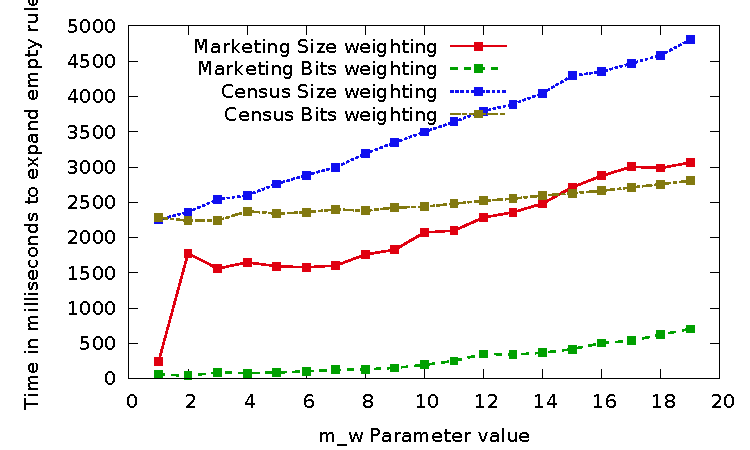
\includegraphics[height=2in]{graphs/mw_speed.pdf}%change height to 2 inch for actual paper, 5 inch for single column
\vspace{-10pt}
  \caption{Running time for different values of parameter $m_w$ \label{fig:mw_speed}}
\vspace{-13pt}
\end{figure}

\subsubsection{Effects of $minSS$}
We now study the effects of the sampling parameter $minSS$. This parameter tells the SampleHandler the minimum sample size on which we run Algorithm~\ref{algo:best-rule-set}.   Higher values of $minSS$ cause our system to use bigger samples, which increases the accuracy of count estimates for displayed rules, but also correspondingly increases computation time. 

We consider one value of $minSS$ and one weight function $W$ at a time. For those values of $minSS$ and $W$, we drill down on the empty rule and measure the time taken for this operation. We also measure the percent error in the estimated counts of the displayed rules. That is, for each displayed rule $r$, if the displayed (estimated) count if $c_1$ and the actual count (computed separately on the entire table) is $c_2$, then the percent error for rule $r$ is $\frac{100 \times |c_1-c_2|}{c_2}$. We consider the average of percent errors over all displayed rules. For each value of $minSS$ and $W$, we drill down on the empty rule and find the computation time and percent error $50$ times, and take the average value for time and error over those $50$ iterations. This average time is plotted against $minSS$, for $W(r) = \text{Size}(r)$ and $W(r) = \sum_{c \in C : r(c) \neq \star} \lceil \text{log}_2(|c|) \rceil$ in Figure~\ref{fig:minSS_speed}. The average percent error is plotted against $minSS$, for $W(r) = \text{Size}(r)$ and $W(r) = \sum_{c \in C : r(c) \neq \star} \lceil \text{log}_2(|c|) \rceil$ in Figure~\ref{fig:minSS_error_percent}. 

The computation time increases approximately linearly with parameter $minSS$. This is expected, because Algorithm~\ref{algo:best-rule-set} makes a constant number of passes over the entire sample, and each pass takes time linear in the size of the sample. The percent error decreases approximately as $\frac{1}{\sqrt{minSS}}$, which is again expected because the standard deviation of estimated $Count$ is approximately inversely proportional to the square root of sample size.
% TODO redo the census bits weighting experiments with proper m_w (forgot to set it correctly earlier)

% TODO, find for census dataset.
In addition, we measure the number of incorrect rules per iteration. If the correct set of rules to display is $r_1, r_2, r_3$ and the displayed set is $r_1, r_3, r_4$ then that means there is one incorrect rule. We find the number of incorrect displayed rules across $50$ iterations, and display the average value in Figure~\ref{fig:minSS_error_rule}. This number is almost always $0$ for the Size weighting function, and between $1$ and $2$ for the Bits weighting function. Note that even when we display an `incorrect' rule, it is usually the $5^{th}$ or $6^{th}$ best rule instead of one of the top $4$ rules, which still results in a reasonably good summary of the table.

\begin{figure}
\hspace{-20pt}
  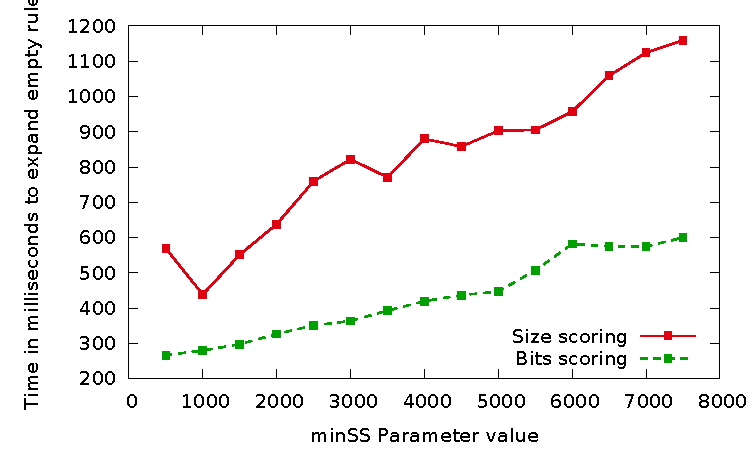
\includegraphics[height=2in]{graphs/minSS_speed.pdf}%change height to 2 inch for actual paper, 5 inch for single column
\vspace{-10pt}
  \caption{Running time for different values of parameter $minSS$ \label{fig:minSS_speed}}
\vspace{-13pt}
\end{figure}

\begin{figure}
\hspace{-20pt}
  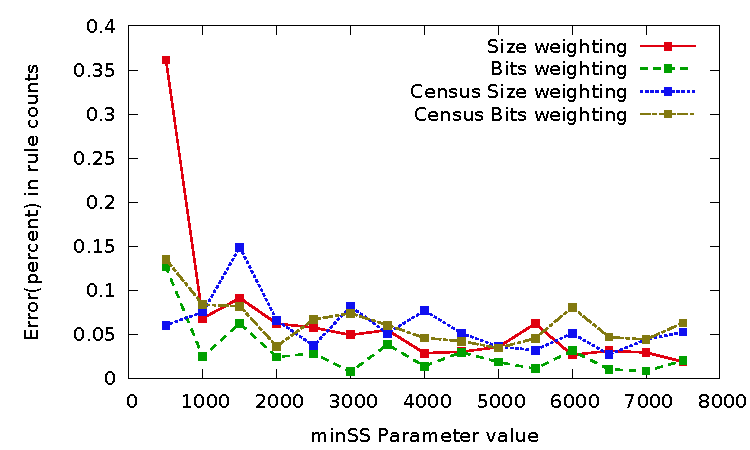
\includegraphics[height=2in]{graphs/minSS_error_percent.pdf}%change height to 2 inch for actual paper, 5 inch for single column
\vspace{-10pt}
  \caption{Error in Count for different values of parameter $minSS$ \label{fig:minSS_error_percent}}
\vspace{-13pt}
\end{figure}

\begin{figure}
\hspace{-20pt}
  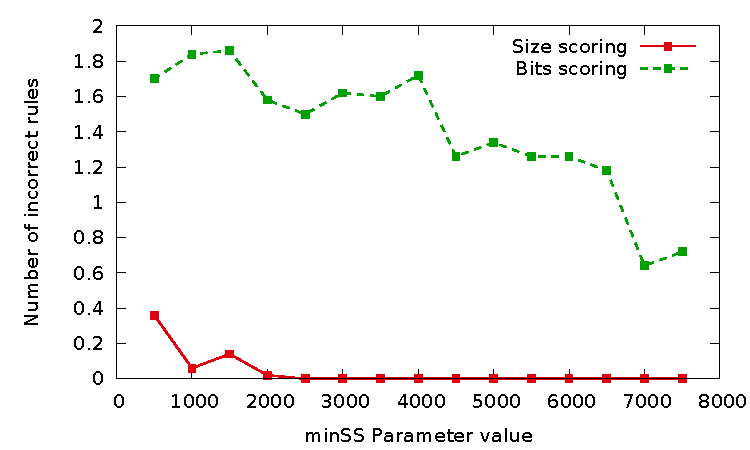
\includegraphics[height=2in]{graphs/minSS_error_rule.pdf}%change height to 2 inch for actual paper, 5 inch for single column
\vspace{-10pt}
\caption{Average number of incorrect rules for different values of parameter $minSS$ \label{fig:minSS_error_rule}}
\vspace{-13pt}
\end{figure}

\begin{comment}
more experiment stuff
vanilla a priori size scoring, first 7 columns (maybe we should include 13, to show suffering on english rule
Female & $\star$ & $\star$ & $\star$ & $\star$ & > 10 years & $2940$ & $2$ \\
$\star$ & $\star$ & $\star$ & $\star$ & $\star$ & > 10 years & $5182$ & $1$ \\
Female & $\star$ & $\star$ & $\star$ & $\star$ & $\star$ & $4918$ & $1$ \\
Male & $\star$ & $\star$ & $\star$ & $\star$ & > 10 years & $2242$ & $2$ \\
$\star$ & Married & $\star$ & $\star$ & $\star$ & > 10 years & $2053$ & $2$ \\
Male & $\star$ & $\star$ & $\star$ & $\star$ & $\star$ & $4075$ & $1$ \\
Female & Married & $\star$ & $\star$ & $\star$ & $\star$ & $1966$ & $2$ \\
$\star$ & Never married & $\star$ & $\star$ & $\star$ & > 10 years & $1964$ & $2$ \\


\end{comment}

\techreporttext{%!TEX root = TableSummarization.tex


\section{Extensions}\label{sec:extensions}
\subsection{Dealing with Numerical Attributes}\label{sec:extensions-numerical}
Our algorithm assumes that all attributes are categorical in nature. Attributes that have a large domain tend to have a smaller tuple count per value, and hence don't appear in rule summaries. Thus our algorithm does not summarise information about numerical attributes. 

However, we can modify the algorithm to deal with numerical attributes. Suppose we have a numerical attribute $A$. A simple approach is to create buckets for values of $A$. We choose a number of buckets $k$, and divide the range of values of $A$ into $k$ intervals, each corresponding to a bucket. We can create buckets having an equal range size, or decide their range such that there is an approximately equal number of tuples in each bucket. Then we can use our algorithm, treating the bucket number as a categorical attribute. This is already done in our MD dataset, where numerical attributes like age are divided into buckets ($18-24$, $25-34$ and so on).

\begin{comment}
The distribution of values for the $A$ may not be similar in different parts of the table. For instance, we may create buckets have approximately equal numbers of tuples in the table. But then suppose a user tries to expand a rule $r$. The part of the table covered by $r$ might have a very different distribution of age values. For instance, in our MD dataset, if the user looks at people who own a house, their age distribution would be different from that of people who are still renting an apartment. To prevent the buckets from getting a skewed distribution when expanding $r$, we could recompute the bucket ranges every time the user expands a rule, and use the new bucket ranges to determine which rules to display upon expansion. 

ask : we should mention this right up front when we're describing the problem.
\end{comment}

\subsection{Using Sum instead of Count}\label{sec:extensions-sum}
Throughout the paper, we define the total score of a rule-list using the marginal counts of rules in the list, and display the count of each rule in our table summary. However, if we have a numerical column (i.e. a `measure' column) in the table, it is straightforward to extend our summary to the `Sum' aggregate over that column instead. Suppose we are given a measure column $c_m$. Then the {\em Sum} for a rule can be defined to be the sum of $c_m$ values over all tuples covered by the rule. {\em MSum} of a rule $r$ in a rule-list $R$ is the sum of $c_m$ values over all tuples covered by $r$ and not covered by any rule in $R$ that occurs before $r$. The Score for $R$ becomes $\text{Score}(R) = \sum_{r\in R} MSum(r,R)W(r)$. Algorithm~\ref{algo:best-rule-set} can be modified to find the best rule set using the new definition of Score, simply by replacing $Count(r)$ by $Sum(r)$ and computing sum and marginal sum instead of count and marginal count in each pass over the table.}

%!TEX root = TableSummarization.tex


\section{Related Work}\label{sec:related}
%TODO: Repeat what we said in intro about interactive, etc.
There has been work on finding cubes to browse in OLAP systems~\cite{Sarawagi:2001:UMA:767141.767148, Sarawagi00user-adaptiveexploration, Sarawagi98discovery-drivenexploration}. This work, along with other existing work~\cite{Mampaey:2011:TMI:2020408.2020499} focuses on finding values that occur more often or less often that expected from a max-entropy distribution. The work does not guarantee good coverage of the table, since it rates infrequently occurring sets of values as highly as frequently occurring ones. 

There is work on constructing `explanation tables', which are sets of rules that co-occur with a given binary attribute of the table~\cite{DBLP:journals/pvldb/GebalyAGKS14}. This work again focuses on displaying rules that will cause the resulting max entropy distribution to best approximate the actual distribution of values. 

Some related work~\cite{Golab_efficientand, Golab:2008:GNT:1453856.1453900} focuses on finding minimum sized Tableaux that provide improved support and confidence for conditional functional dependencies. There has also been work~\cite{Bu:2005:MSH:1083592.1083644, Lakshmanan:2002:GMA:1287369.1287435, Xiang_succinctsummarization, Geerts04tilingdatabases} on finding hyper-rectangle based covers for tables. In both these cases, the emphasis is on completely covering or 
summarizing the table, suffering from the same problems as traditional drill down in that the user may be presented with
too many results. The techniques in the former case may end up picking rare ``patterns'' if they have high confidence, and in the latter case do not scale well to a large number of attributes (in their case, $\geq 4$). 

Several existing papers also deal with the problem of frequent itemset mining~\cite{apriori, 1411744, Han:2000:MFP:342009.335372}. Vanilla frequent itemset mining is not directly applicable to our problem because the flexible user-specified objective function emphasizes coverage of the table rather than simply frequent itemsets.  However, we do leverage ideas from the a-priori algorithm~\cite{apriori} as applicable. Several extensions have been proposed to the a-priori algorithm, including those for dealing with numerical attributes~\cite{Srikant:1996:MQA:233269.233311, Miller:1997:ARO:253260.253361}. We can potentially use these ideas to improve handing of numerical attributes in our work. Unlike our paper, there has been no work on dynamically maintaining samples for interaction in the frequent itemset literature, since frequent itemset mining is a one-shot problem.

% All the existing works solve a fixed optimization problem, whereas  we focus on finding an optimal summary for a flexible user-specified weighting function.

We use sampling to find approximate estimates of rule counts. Various other database systems~\cite{Acharya:1999:AAQ:304182.304581, Agarwal:2013:BQB:2465351.2465355} use samples to find approximate results to SQL aggregation queries. These systems create samples in advance and only update them when the database changes. In contrast, we keep updating our samples on the fly, as the user interacts with our system. 

% Our algorithm uses ideas from the a priori algorithm~\cite{apriori}. 

% Related Work summary : Is ours the only only that is flexible (due to weight function black box)?
% Explanation tables takes lots of papers and talks about them in one go in related work. saying they optimize for different opbjective functions. We can say that as well. We have a unique idea of flexible weighting functions for managing the tradeoff between coverage and specificity. 
% Succintly summarizing with itemsets-- Mampaey:2011:TMI:2020408.2020499 -- Also seemed to optimize according to max entropy criterion
% Efficient and Effective... Tableaux -- Golab_efficientand -- Similar to conditional functional dep. paper.
% Near Optimal Tableaux Conditional functional dep. -- Golab:2008:GNT:1453856.1453900 -- Finding a smallest sized tableau that provides some confidence and support for a conditional functional dependency.
% MDL Summarization with holes -- Bu:2005:MSH:1083592.1083644 -- Min sized summary with a rectangle and exceptions (holes). 
% Generalized MDL Approach -- Lakshmanan:2002:GMA:1287369.1287435 -- Similar to MDL Approach.
% Overlapped Hyperrectangle -- Xiang_succinctsummarization -- Efficiently find the set of hyperrectangles that covers the data (sets of itemsets)
% Tiling Databases Geerts04tilingdatabases Simlar to hyper-rectangles. Probabilistic interpretation of frequent itemsets. 



%!TEX root = smartDrillDownICDE.tex

\section{Conclusion}\label{sec:conclusion}
We have presented a new data exploration operator called smart drill down.
Like traditional drill down, it allows an analyst
to quickly discover interesting value patterns (rules) that occur frequently
(or that represent high values of some metric attribute)
across diverse parts of a table.

We presented an algorithm for optimally selecting rules
to display, as well as a scheme for performing such selections
based on data samples. Working with samples makes smart drill down
relatively insensitive to the size of the table.

Our experimental results on our experimental prototype show that smart drill down
is fast enough to be interactive under various
realistic scenarios. We also showed that the accuracy is high
when sampling is used, and when the maximum weight ($m_w$)
approximation is used. Moreover, we have a tunable parameter $minSS$ that the user can tweak to tradeoff performance of smart drill down for the accuracy of the rules.

\balance
{\small
\bibliographystyle{abbrv}
\bibliography{TableSummarization}  
}

% Example of an appendix; typically would start on a new page
%pagebreak

\techreporttext{\input{appendix}}

\end{document}
